\documentclass{report}
\usepackage[spanish]{babel}
\usepackage[utf8]{inputenc}
\usepackage{graphicx, longtable, float, titlesec, hyperref, array, listings}

\hypersetup{
    hidelinks = true
}

\titleformat{\chapter}[display]
  {\normalfont\bfseries}{}{0pt}{\Huge}

\begin{document}
    \begin{titlepage}
        \centering
        
\includegraphics[width=0.6\textwidth]{./img/portada/logo.jpg}\\
        \vspace{1cm}
        \LARGE Análisis y Diseño de Sistemas de Información\\
        \vspace{0.5cm}
        \Large Ingeniería Informática de Gestión y Sistemas de Información\\
        \vspace{3cm}
        \Huge Biblioteca\\
        \vspace{2.5cm}
        \Large Autores:\\
        \vspace{0.2cm}
        \large Xabier Gabiña Barañano\\
        \large Janire Veganzones García\\
        \large Ainhize Martinez Duran\\
        \large Javier Criado Garcia\\
        \large Kepa Reches Urrutia\\
        \large Jon Valdes Granado\\
        \large Mohamed El Basri Dehbi\\
        \vfill
        \today
    \end{titlepage}

    \tableofcontents
    \chapter{Changelog}
        \section{Versión 1 (2023-10-08)}
            \begin{itemize}
                \item Añadido caso de uso general.
                \item Añadidos los casos de uso extendidos.
            \end{itemize}  
        \section{Versión 2 (2023-10-22)}
            \begin{itemize}
                \item Añadido modelo de dominio.
                \item Modificado el caso de uso general.
                \item Modificados los casos de uso extendidos.
            \end{itemize}
        \section{Versión 3 (2023-11-05)}
            \begin{itemize}
                \item Añadido plan de Pruebas.
                \item Modificado el modelo de dominio.
            \end{itemize}
        \section{Versión 4 (2023-11-15)}
            \begin{itemize}
                \item Añadido diagrama relacional.
                \item Añadido diagrama de clases.
                \item Añadido diagrama de comunicación.
            \end{itemize}
    \chapter{Introducción}
    En un mundo cada vez más digitalizado, las bibliotecas modernas están buscando formas innovadoras de adaptarse a las necesidades cambiantes de sus usuarios. La biblioteca que nos ocupa se encuentra en este proceso de transformación, reconociendo la importancia de expandir sus servicios en línea y brindar a sus usuarios una experiencia más enriquecedora y conectada. Para llevar a cabo esta ambiciosa misión, han solicitado la colaboración de nuestro equipo de desarrollo.\\
    En su estado actual, la biblioteca cuenta con un servicio web que permite a los usuarios consultar su extenso catálogo de libros. Además, ofrece un apartado de usuarios que pueden acceder a una sección privada. Sin embargo, esta plataforma carece de funcionalidades adicionales que pueden mejorar significativamente la experiencia de los usuarios y promover una mayor interacción entre ellos.\\
    En este proyecto, nuestro objetivo es expandir y mejorar el servicio web de la biblioteca, dotándolo de una serie de funcionalidades clave. Estas nuevas características incluyen la gestión de reservas, la capacidad de dejar reseñas y comentarios en los libros, la creación de una red de amigos entre los usuarios, la introducción de un rol de administrador con capacidades de gestión, la implementación de foros para discusión y la incorporación de sistemas de recomendación, tanto basados en el historial de lecturas como en la afinidad de intereses entre usuarios.\\
    A lo largo de este documento, exploraremos en detalle cada una de estas funcionalidades, presentando soluciones técnicas y estratégicas para su implementación. Este proyecto representa una emocionante oportunidad para ayudar a la biblioteca a evolucionar y brindar un servicio en línea más completo y enriquecedor a su comunidad de usuarios ávidos de conocimiento y lectura.\\
    \chapter{Casos de Uso}
        \section{General}
            \begin{figure}[H]
                \centering
                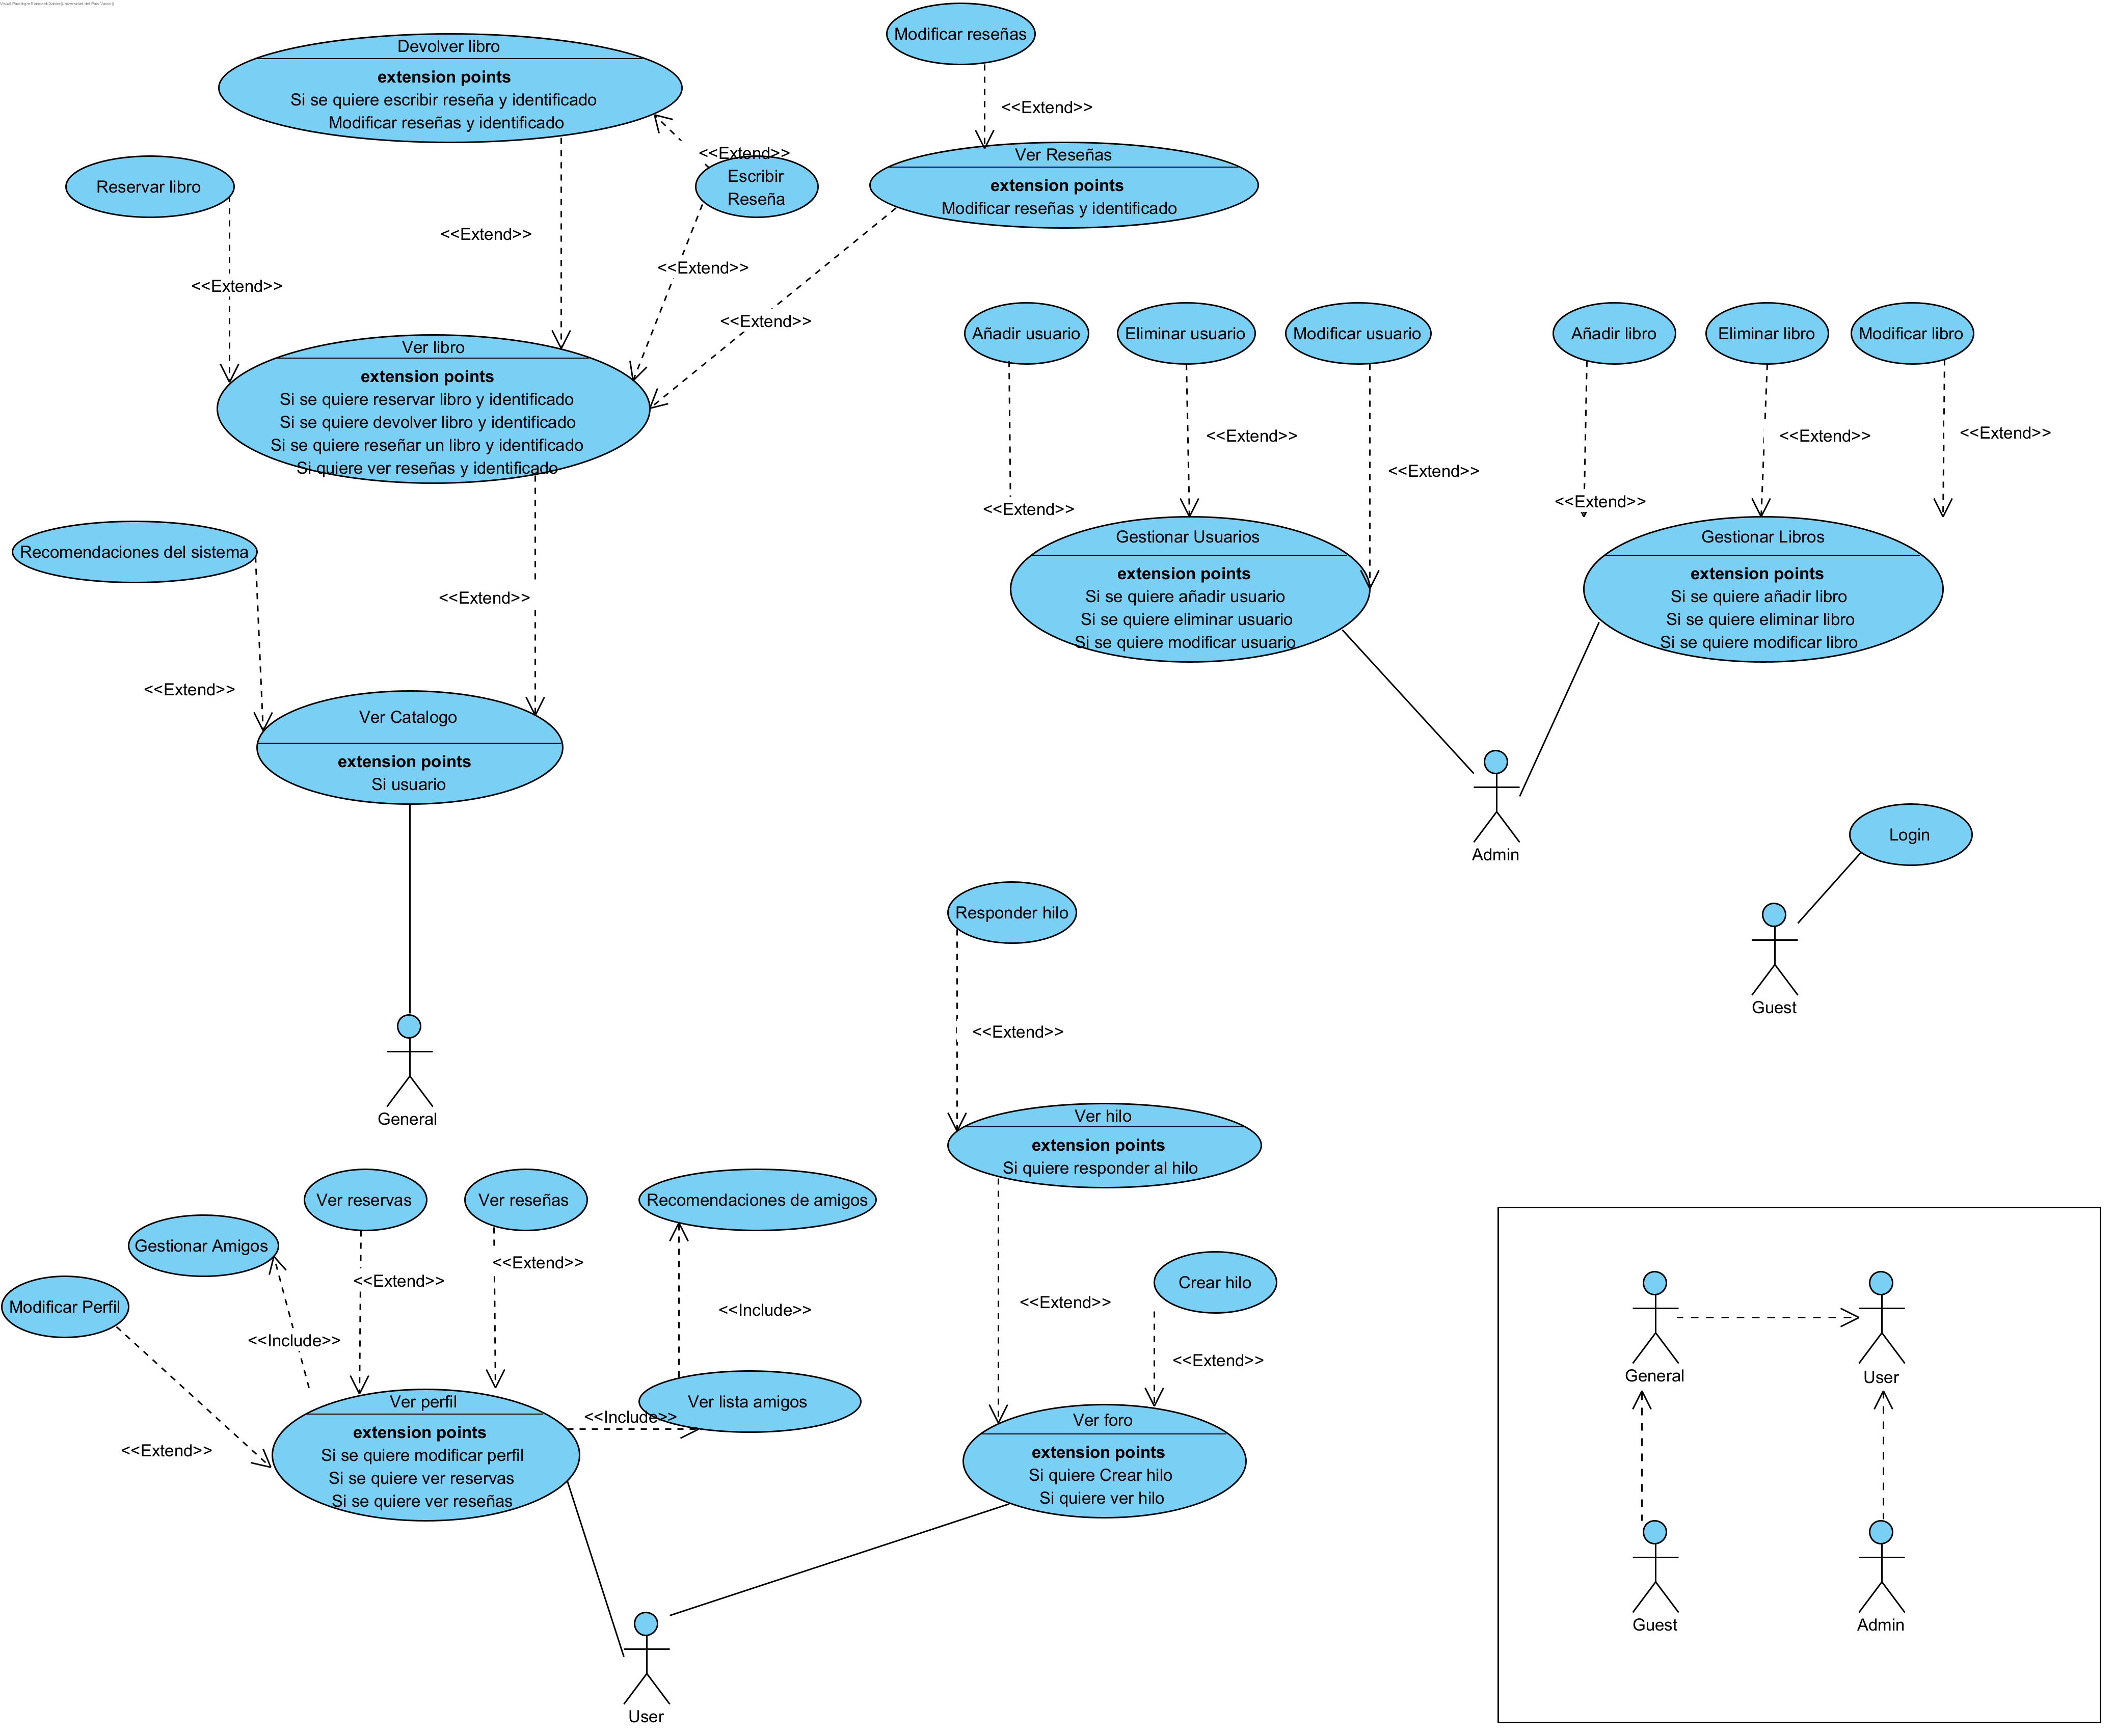
\includegraphics[scale=0.3]{img/casos_uso/General.png}
                \caption{Diagrama de casos de uso general}
            \end{figure}
        \clearpage
        \section{Extendidos}
            \subsection{Gestión de reservas}
                \begin{center}
                    \begin{longtable}{|p{\linewidth}|}
                        \hline
                        \textbf{Responsable:} Mohamed El Basri\\
                        \hline
                        \begin{figure}[H]
                            \centering
                            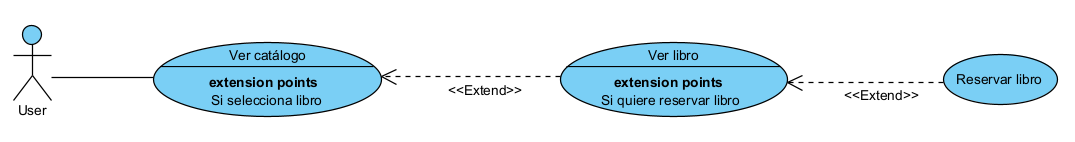
\includegraphics[width=0.8\textwidth]{./img/casos_uso/GestionDeReservas.png}
                            \\Figura 3.2.1.1: Diagrama de casos de uso de la subfuncionalidad de gestión de reservas
                        \end{figure}\\
                        \hline
                        \textbf{Nombre:} Ver libros recomendados\\
                        \hline
                        \textbf{Descripción:} Permite a los usuarios realizar reservas de libros.\\
                        \hline
                        \textbf{Actores:} Usuario\\
                        \hline
                        \textbf{Precondiciones:} Estar identificado en el sistema.\\
                        \hline
                        \textbf{Requisitos no funcionales:} Ninguno\\
                        \hline
                        \textbf{Flujo de Eventos:}
                        \begin{enumerate}
                            \item El usuario selecciona el libro deseado en el catálogo y pulsa “Reservar”. Se abre la interfaz de reserva (Figura 3.2.1.2).
                            \item Si el usuario pulsa aceptar, si el tiempo de reserva es menor a 2 meses aparece una interfaz indicando que la reserva se ha realizado con éxito (Figura 3.2.1.3).
                            \begin{enumerate}
                                \item Si el usuario pulsa aceptar, si el tiempo de reserva es mayor a 2 meses aparece una interfaz indicando error (Figura 3.2.1.4).
                                \item Si el usuario pulsa cancelar, se cierra la interfaz.
                            \end{enumerate}
                        \end{enumerate}\\
                        \hline
                        \textbf{Poscondiciones:} Ninguna\\
                        \hline
                        \textbf{Interfaz Gráfica:}\\
                        \begin{figure}[H]
                            \centering
                            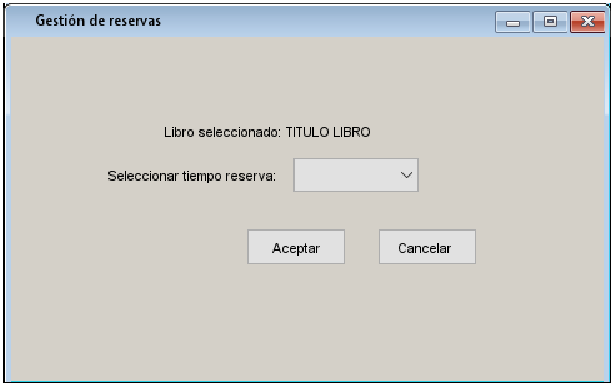
\includegraphics[width=0.8\textwidth]{./img/grafico/GestionDeReservas1.PNG}
                            \\Figura 3.2.1.2: Interfaz de reserva
                        \end{figure}\\
                        \begin{figure}[H]
                            \centering
                            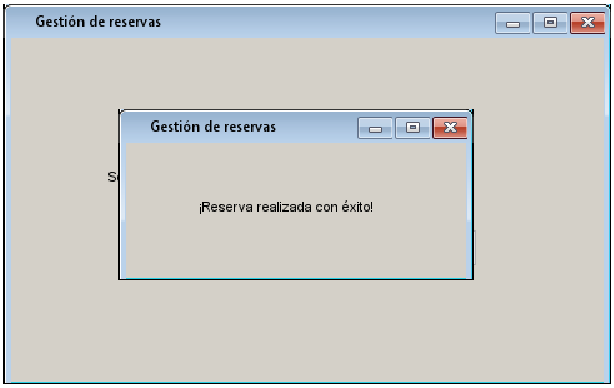
\includegraphics[width=0.8\textwidth]{./img/grafico/GestionDeReservas2.PNG}
                            \\Figura 3.2.1.3: Interfaz de reserva con éxito
                        \end{figure}\\
                        \begin{figure}[H]
                            \centering
                            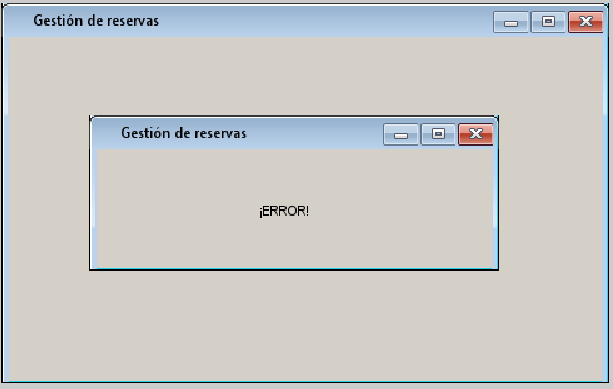
\includegraphics[width=0.8\textwidth]{./img/grafico/GestionDeReservas3.PNG}
                            \\Figura 3.2.1.4: Interfaz de reserva con error
                        \end{figure}\\
                        \hline
                    \end{longtable}
                \end{center}
            \clearpage
            \subsection{Reseñas}
                \begin{center}
                    \begin{longtable}{|p{\linewidth}|}
                        \hline
                        \textbf{Responsable:} Javier Criado\\
                        \hline
                        \begin{figure}[H]
                            \centering
                            \includegraphics[width=0.8\textwidth]{./img/casos_uso/Reseñas.png}
                            \\Figura 3.2.2.1: Diagrama de casos de uso de la subfuncionalidad de reseñas
                        \end{figure}\\
                        \hline
                        \textbf{Nombre:} Reseñas\\
                        \hline
                        \textbf{Descripción:} Permite al cliente puntuar y comentar en un libro una vez lo haya devuelto, también permite modificar estos datos posteriormente.\\
                        \hline
                        \textbf{Actores:} Usuario\\
                        \hline
                        \textbf{Precondiciones:} Estar identificado en el sistema\\
                        \hline
                        \textbf{Requisitos no funcionales:} Ninguno\\
                        \hline
                        \textbf{Flujo de Eventos:}
                        \begin{enumerate}
                            \item El usuario entra en el catalogo para ver los libros disponibles.
                            \begin{enumerate}
                                \item El usuario selecciona uno de los libros. [Figura 3.2.2.2]
                                \begin{enumerate}
                                    \item Al seleccionar 'Devolver libro', se devolvera el libro y se podra añadir una nueva reseña.
                                    \item Al seleccionar 'Escribir reseña', se abrira una pestaña donde se podrá escribir una reseña sobre el libro. [Figura 3.2.2.3]
                                    \item Al seleccionar el boton 'Ver reseñas', el usuario podrá ver las reseñas sobre el libro. [Figura 3.2.2.4]
                                    \begin{enumerate}
                                        \item Al hacer click sobre una de las reseñas esta se mostrara en una ventana aparte. [Figura 3.2.2.5]
                                    \end{enumerate}
                                \end{enumerate} 
                            \end{enumerate} 
                        \end{enumerate}\\
                        \hline
                        \textbf{Poscondiciones:} Ninguna\\
                        \hline
                        \textbf{Interfaz Gráfica:}\\
                        \begin{figure}[H]
                            \centering
                            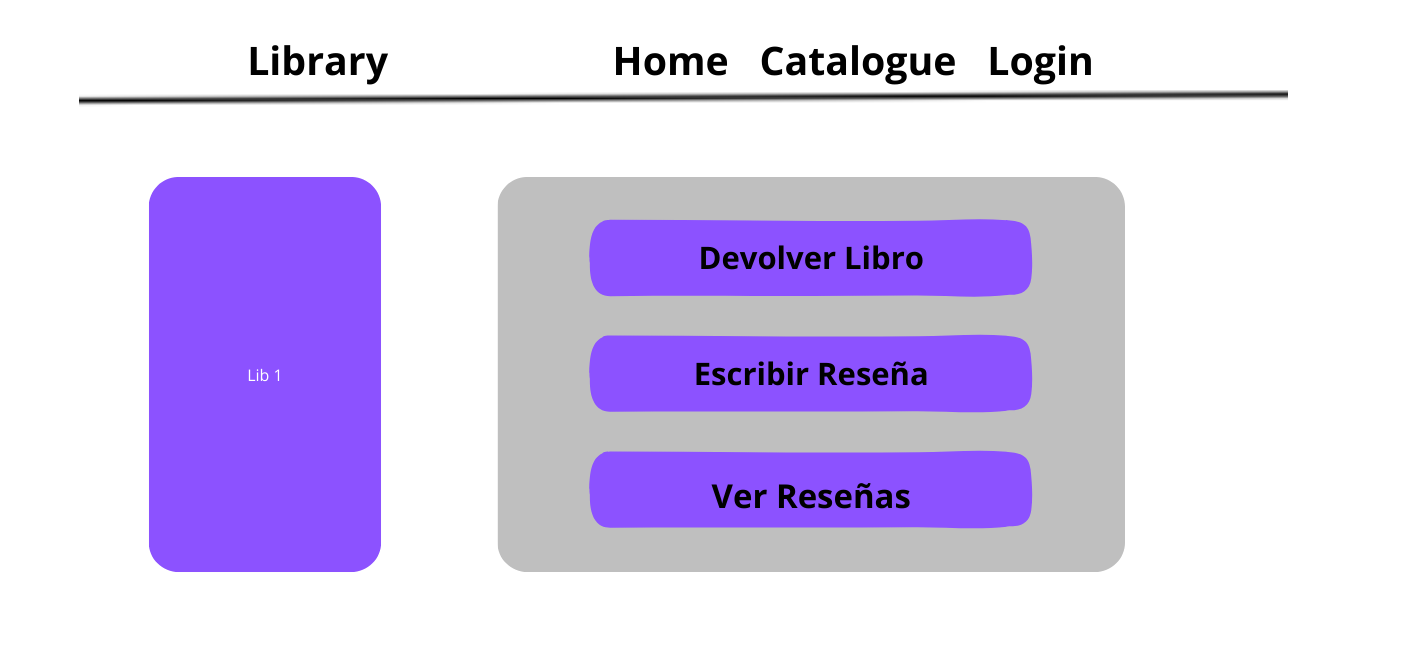
\includegraphics[width=0.8\textwidth]{./img/grafico/Ver_Libro.png}
                            \\Figura 3.2.2.2: Interfaz de ver libro.
                        \end{figure}\\
                        \begin{figure}[H]
                            \centering
                            \includegraphics[width=0.8\textwidth]{./img/grafico/Escribir_Reseña.png}
                            \\Figura 3.2.2.3: Interfaz de escribir reseña.
                        \end{figure}\\
                        \begin{figure}[H]
                            \centering
                            \includegraphics[width=0.8\textwidth]{./img/grafico/Ver_Reseñas.jpg}
                            \\Figura 3.2.2.4: Interfaz para ver las reseñas.
                        \end{figure}\\
                        \begin{figure}[H]
                            \centering
                            \includegraphics[width=0.8\textwidth]{./img/grafico/Ver_Una_Reseña.jpg}
                            \\Figura 3.2.2.5: Interfaz para ver una reseña.
                        \end{figure}\\
                        \hline
                    \end{longtable}
                \end{center}
                \clearpage
            \subsection{Red de amigos}
                \begin{center}
                    \begin{longtable}{|p{\linewidth}|}
                        \hline
                        \textbf{Responsable:} Jon Valdes\\
                        \hline
                        \begin{figure}[H]
                            \centering
                            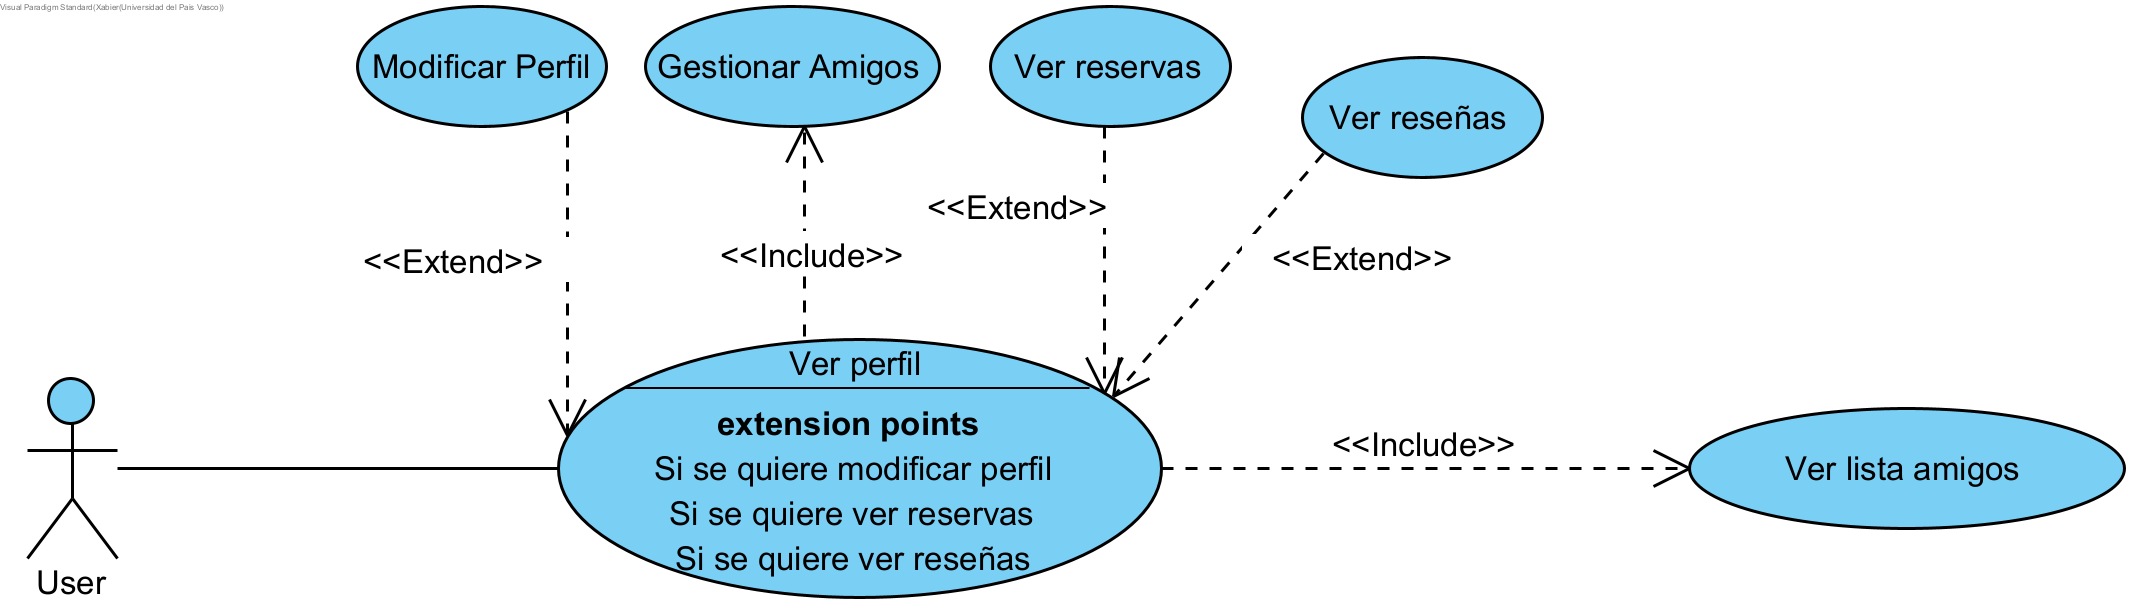
\includegraphics[width=0.8\textwidth]{./img/casos_uso/RedAmigos.png}
                            \\Figura 3.2.3.1: Diagrama de casos de uso de la subfuncionalidad de red de amigos
                        \end{figure}\\
                        \hline
                        \textbf{Nombre:} Red de amigos.\\
                        \hline
                        \textbf{Descripción:} Permite al usuario gestionar su perfil, de modo que puede tanto consultar el historial de reservas y de reseñas, como añadir o eliminar amigos. También puede editar sus datos personales.\\
                        \hline
                        \textbf{Actores:} Usuario.\\
                        \hline
                        \textbf{Precondiciones:} Estar identificado en el sistema.\\
                        \hline
                        \textbf{Requisitos no funcionales:} Ninguno\\
                        \hline
                        \textbf{Flujo de Eventos:}
                        \begin{enumerate}
                            \item El usuario accede a su perfil. [Figura 3.2.3.2]
                            \begin{enumerate}
                                \item El usuario puede pulsar 'Editar perfil' para editar sus datos. [Figura 3.2.3.5]
                                \item El usuario puede pulsar 'Consultar reservas' para ver su historial de reservas.
                                \item El usuario puede pulsar 'Consultar reseñas' para ver su historial de reseñas.
                                \item El usuario puede ver su lista de amigos.
                                \item El usuario puede pulsar 'Añadir amigo' para añadir un amigo. [Figura 3.2.3.3]
                                \item El usuario puede pulsar 'Solicutudes de amistad' para ver las solicitudes de amistad pendientes.
                                \item El usuario puede pulsar 'Eliminar amigo' para eliminar un amigo. [Figura 3.2.3.4]
                            \end{enumerate}
                        \end{enumerate}\\
                        \hline
                        \textbf{Poscondiciones:} Ninguna\\
                        \hline
                        \textbf{Interfaz Gráfica:}\\
                        \begin{figure}[H]
                            \centering
                            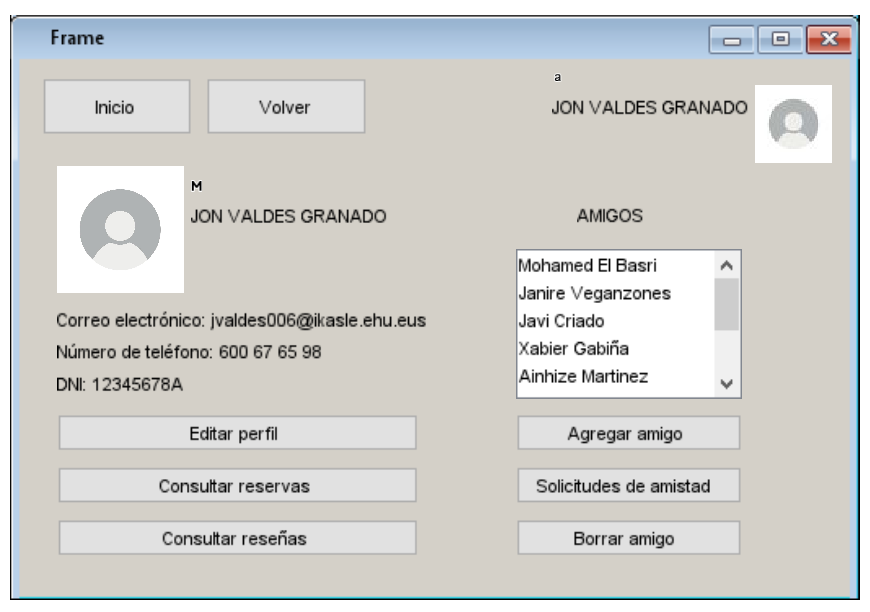
\includegraphics[width=0.8\textwidth]{./img/grafico/InterfazMenu.png}
                            \\Figura 3.2.3.2: Interfaz del perfil de usuario.
                        \end{figure}\\
                        \begin{figure}[H]
                            \centering
                            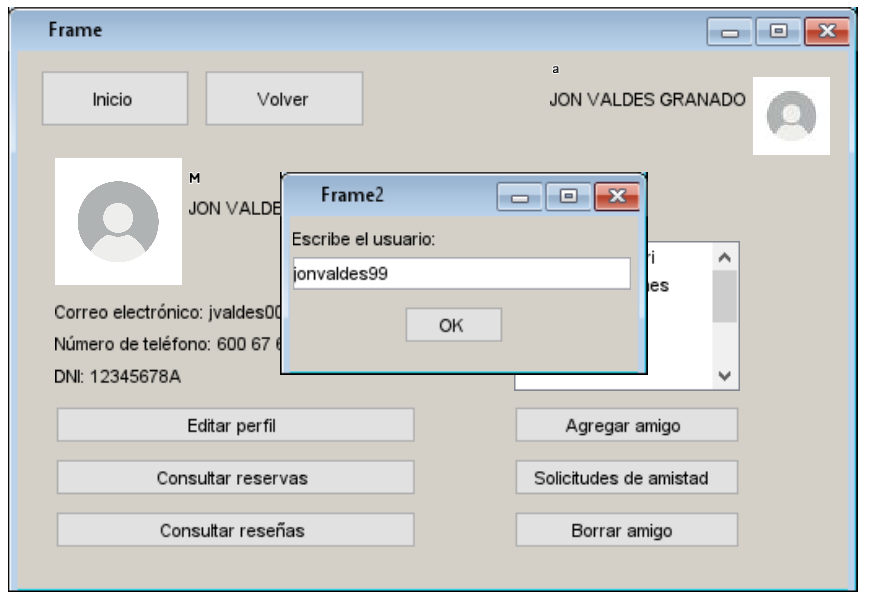
\includegraphics[width=0.8\textwidth]{./img/grafico/InterfazAnadrAmigo.png}
                            \\Figura 3.2.3.3: Interfaz para añadir un amigo.
                        \end{figure}\\
                        \begin{figure}[H]
                            \centering
                            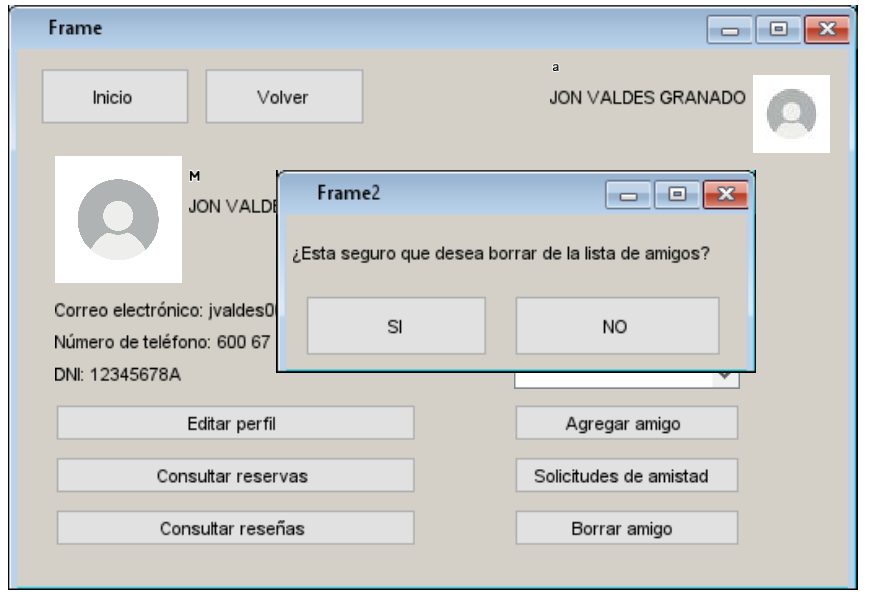
\includegraphics[width=0.8\textwidth]{./img/grafico/interfazAlertaBorrarAmigo.png}
                            \\Figura 3.2.3.4: Interfaz de alerta para borrar un amigo.
                        \end{figure}\\
                        \begin{figure}[H]
                            \centering
                            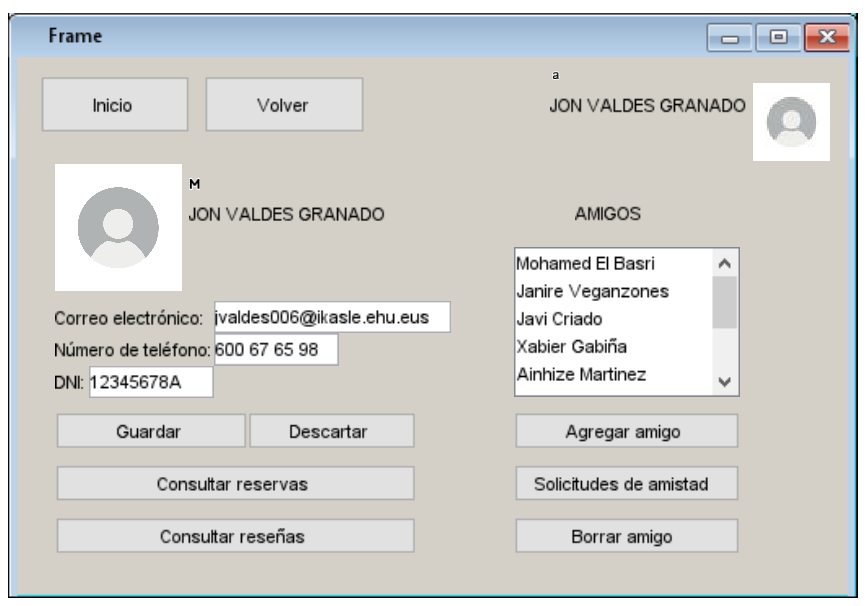
\includegraphics[width=0.8\textwidth]{./img/grafico/InterfazEditarPerfil.png}
                            \\Figura 3.2.3.5: Interfaz para editar el perfil.
                        \end{figure}\\
                        \hline
                    \end{longtable}
                \end{center}
                \clearpage
            \subsection{Administrador}
                \subsubsection*{Gestión de usuarios}
                    \begin{center}
                        \begin{longtable}{|p{\linewidth}|}
                            \hline
                            \textbf{Responsable:} Janire Veganzones\\
                            \hline
                            \begin{figure}[H]
                                \centering
                                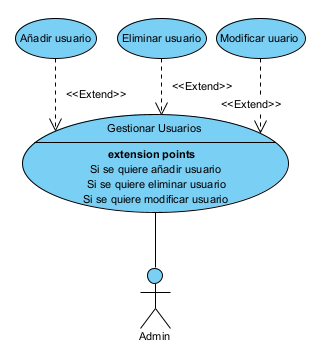
\includegraphics[width=0.45\textwidth]{./img/casos_uso/GestionarUsuarios.png}
                                \\Figura 3.2.4.1.1: Diagrama de casos de uso de la subfuncionalidad de gestión de usuarios
                            \end{figure}\\
                            \hline
                            \textbf{Nombre:} Gestionar usuarios\\
                            \hline
                            \textbf{Descripción:}  Permite crear, eliminar o modificar un usuario en el sistema.\\
                            \hline
                            \textbf{Actores:} Admin\\
                            \hline
                            \textbf{Precondiciones:} Estar identificado en el sistema y ser administrador.\\
                            \hline
                            \textbf{Requisitos no funcionales:} Ninguno\\
                            \hline
                            \textbf{Flujo de Eventos:}
                            \begin{enumerate}
                                \item Se accede al menu de administrador. [Figura 3.2.4.1.2]
                                \begin{enumerate}
                                    \item Se selecciona la opción de gestionar usuarios. [Figura 3.2.4.1.3]
                                    \begin{enumerate}
                                        \item El administrador pulsa 'Crear' para crear un nuevo usuario. [Figura 3.2.4.1.4]
                                        \begin{enumerate}
                                            \item Si hay un error al crear un usuario saldra un error mostrandolo. [Figura 3.2.4.1.5]
                                        \end{enumerate}
                                        \item El administrador pulsa 'Borrar' para borrar un usuario. [Figura 3.2.4.1.6]
                                        \begin{enumerate}
                                            \item Si el usuario a borrar no existe mostrara un error. [Figura 3.2.4.1.7]
                                        \end{enumerate}
                                        \item El administrador pulsa 'Modificar' para modificar un usuario. [Figura 3.2.4.1.8]
                                        \begin{enumerate}
                                            \item Si hay un error al modificar un usuario saldra un error mostrandolo. [Figura 3.2.4.1.9]
                                        \end{enumerate}
                                    \end{enumerate}
                                \end{enumerate} 
                            \end{enumerate}\\
                            \hline
                            \textbf{Poscondiciones:} Ninguna\\
                            \hline
                            \textbf{Interfaz Gráfica:}\\
                            \begin{figure}[H]
                                \centering
                                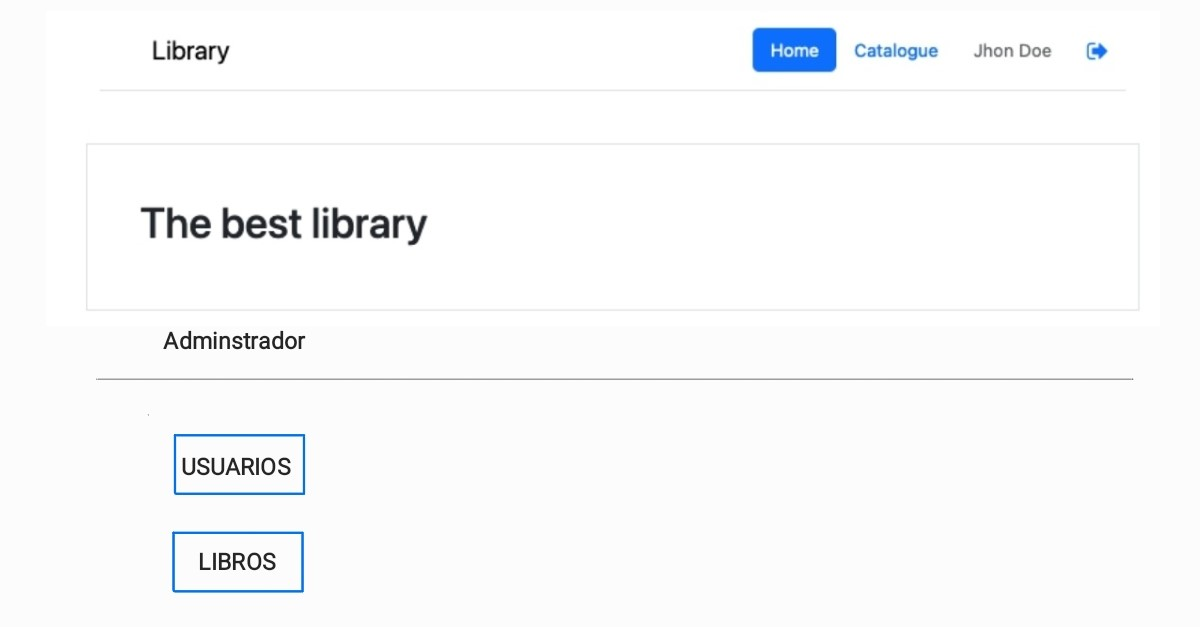
\includegraphics[width=0.8\textwidth]{./img/grafico/MenuAdmin.jpg}
                                \\Figura 3.2.4.1.2: Interfaz del menú de administrador.
                            \end{figure}\\
                            \begin{figure}[H]
                                \centering
                                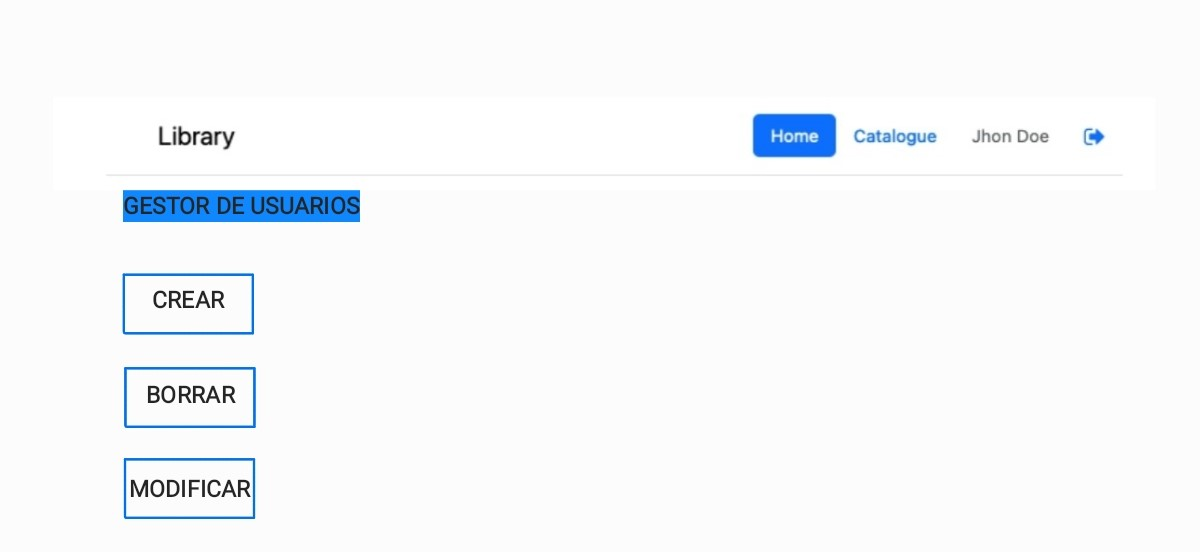
\includegraphics[width=0.8\textwidth]{./img/grafico/MenuGestorUsu.jpg}
                                \\Figura 3.2.4.1.3: Interfaz del menu de gestión de usuarios.
                            \end{figure}\\
                            \begin{figure}[H]
                                \centering
                                \includegraphics[width=0.8\textwidth]{./img/grafico/AñadirUsu.jpg}
                                \\Figura 3.2.4.1.4: Interfaz para añadir un usuario.
                            \end{figure}\\
                            \begin{figure}[H]
                                \centering
                                \includegraphics[width=0.8\textwidth]{./img/grafico/ErrorAñadirUsu.jpg}
                                \\Figura 3.2.4.1.5: Interfaz de error al añadir un usuario.
                            \end{figure}\\
                            \begin{figure}[H]
                                \centering
                                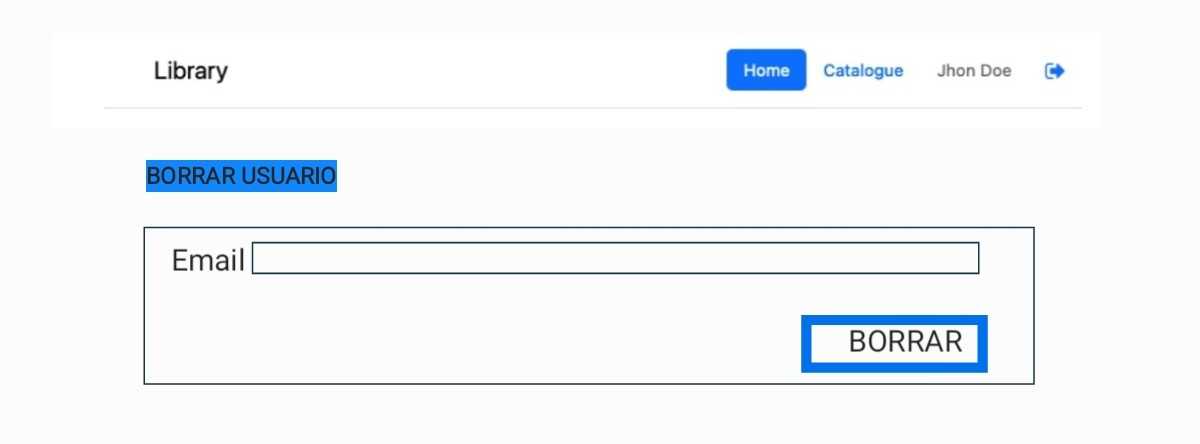
\includegraphics[width=0.8\textwidth]{./img/grafico/BorrarUsu.jpg}
                                \\Figura 3.2.4.1.6: Interfaz para borrar un usuario.
                            \end{figure}\\
                            \begin{figure}[H]
                                \centering
                                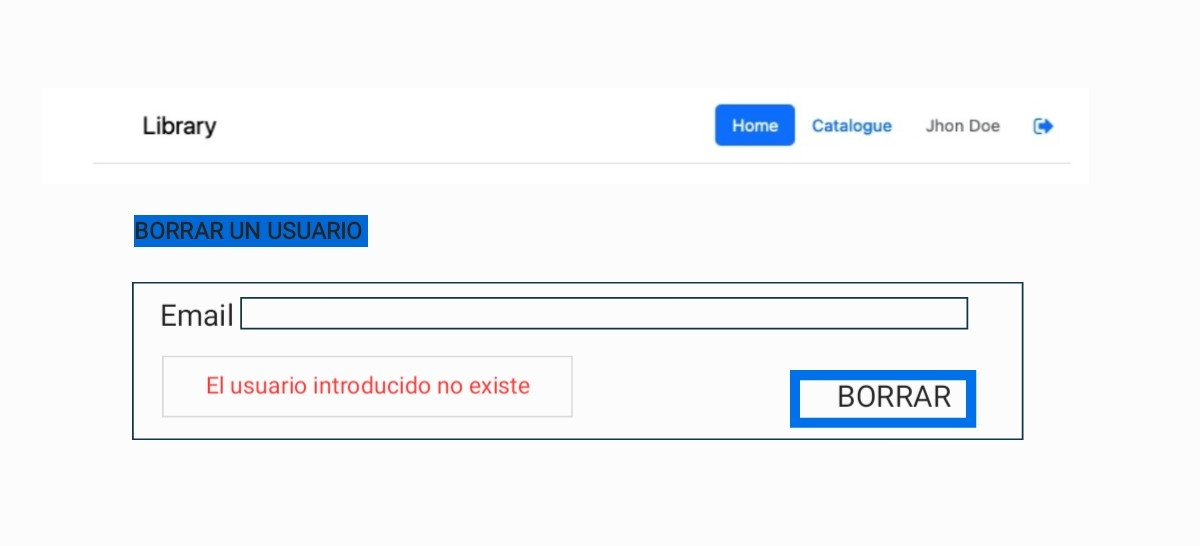
\includegraphics[width=0.8\textwidth]{./img/grafico/ErrorBorrarUsu.jpg}
                                \\Figura 3.2.4.1.7: Interfaz de error al borrar un usuario.
                            \end{figure}\\
                            \begin{figure}[H]
                                \centering
                                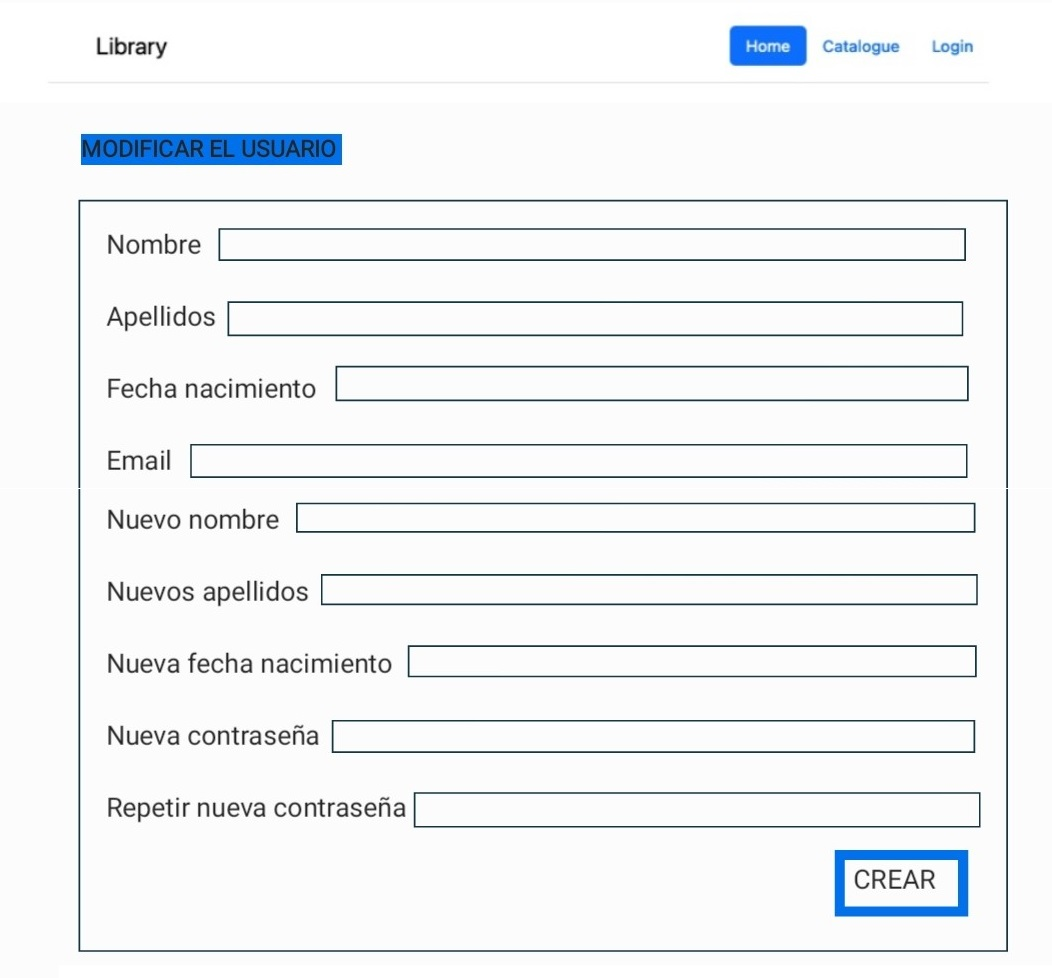
\includegraphics[width=0.8\textwidth]{./img/grafico/ModificarUsu.jpg}
                                \\Figura 3.2.4.1.8: Interfaz para modificar un usuario.
                            \end{figure}\\
                            \begin{figure}[H]
                                \centering
                                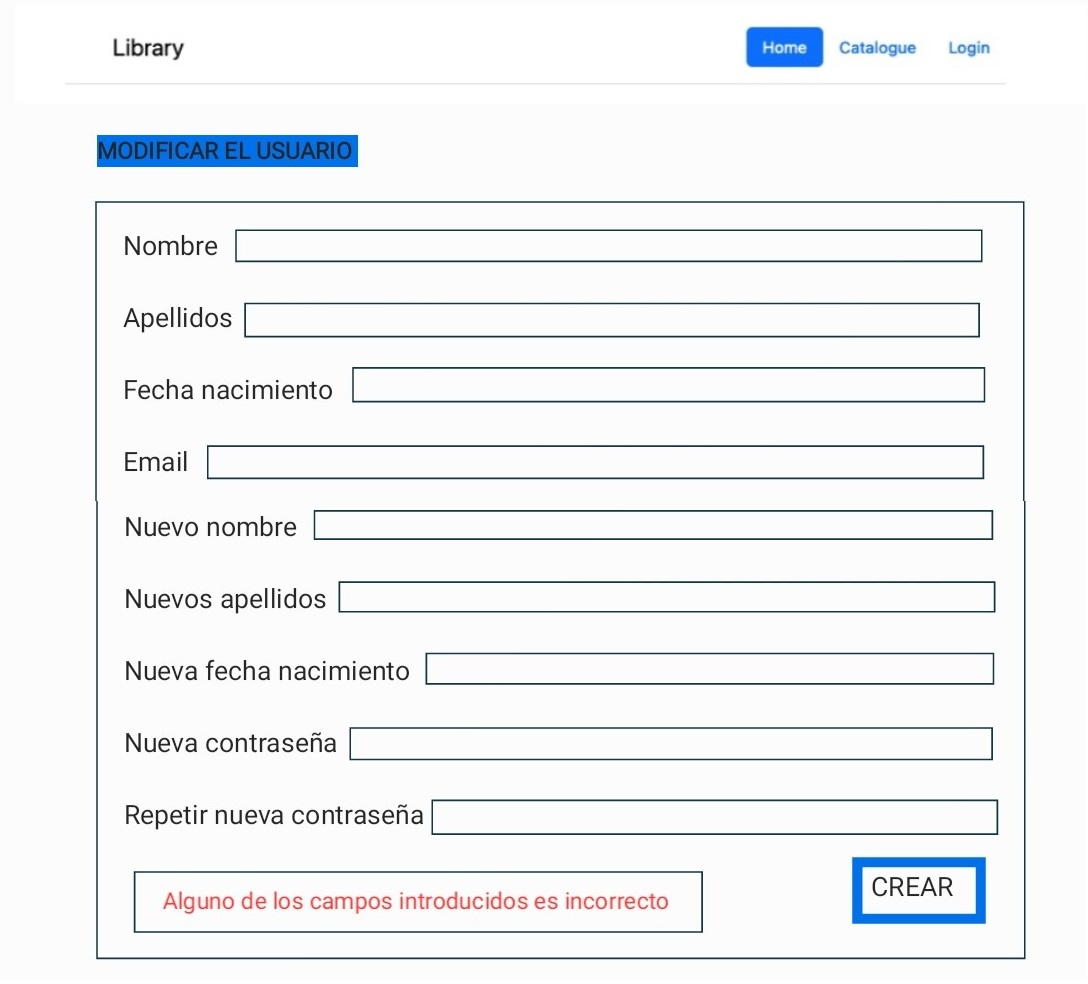
\includegraphics[width=0.8\textwidth]{./img/grafico/ErrorModificarUsu.jpg}
                                \\Figura 3.2.4.1.9: Interfaz de error al modificar un usuario.
                            \end{figure}\\
                            \hline
                        \end{longtable}
                    \end{center}
                    \clearpage
                \subsubsection*{Gestión de libros}
                    \begin{center}
                        \begin{longtable}{|p{\linewidth}|}
                            \hline
                            \textbf{Responsable:} Janire Veganzones\\
                            \hline
                            \begin{figure}[H]
                                \centering
                                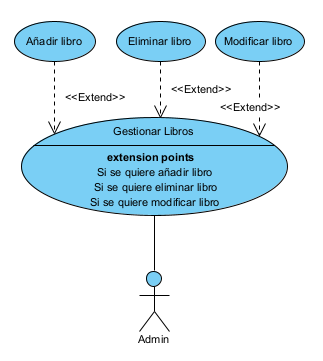
\includegraphics[width=0.45\textwidth]{./img/casos_uso/GestionarLibros.png}
                                \\Figura 3.2.4.2.1: Diagrama de casos de uso de la subfuncionalidad de gestión de libros
                            \end{figure}\\
                            \hline
                            \textbf{Nombre:} Gestionar libros\\
                            \hline
                            \textbf{Descripción:}  Permite añadir, eliminar o modificar un libro en el sistema.\\
                            \hline
                            \textbf{Actores:} Admin\\
                            \hline
                            \textbf{Precondiciones:} Estar identificado en el sistema y ser usuario.\\
                            \hline
                            \textbf{Requisitos no funcionales:} Ninguno\\
                            \hline
                            \textbf{Flujo de Eventos:}
                            \begin{enumerate}
                                \item Se accede al menu de administrador. [Figura 3.2.4.2.2]
                                \begin{enumerate}
                                    \item Se selecciona la opción de gestionar libros. [Figura 3.2.4.2.3]
                                    \begin{enumerate}
                                        \item El administrador pulsa 'Crear' para crear un nuevo libro. [Figura 3.2.4.2.4]
                                        \begin{enumerate}
                                            \item Si hay un error al crear un libro saldra un error mostrandolo. [Figura 3.2.4.2.5]
                                        \end{enumerate}
                                        \item El administrador pulsa 'Borrar' para borrar un libro. [Figura 3.2.4.2.6]
                                        \begin{enumerate}
                                            \item Si el libro a borrar no existe mostrara un error. [Figura 3.2.4.2.7]
                                        \end{enumerate}
                                        \item El administrador pulsa 'Modificar' para modificar un libro. [Figura 3.2.4.2.8]
                                        \begin{enumerate}
                                            \item Si hay un error al modificar un libro saldra un error mostrandolo. [Figura 3.2.4.2.9]
                                        \end{enumerate}
                                    \end{enumerate}
                                \end{enumerate} 
                            \end{enumerate}\\
                            \hline
                            \textbf{Poscondiciones:} Ninguna\\
                            \hline
                            \textbf{Interfaz Gráfica:}\\
                            \begin{figure}[H]
                                \centering
                                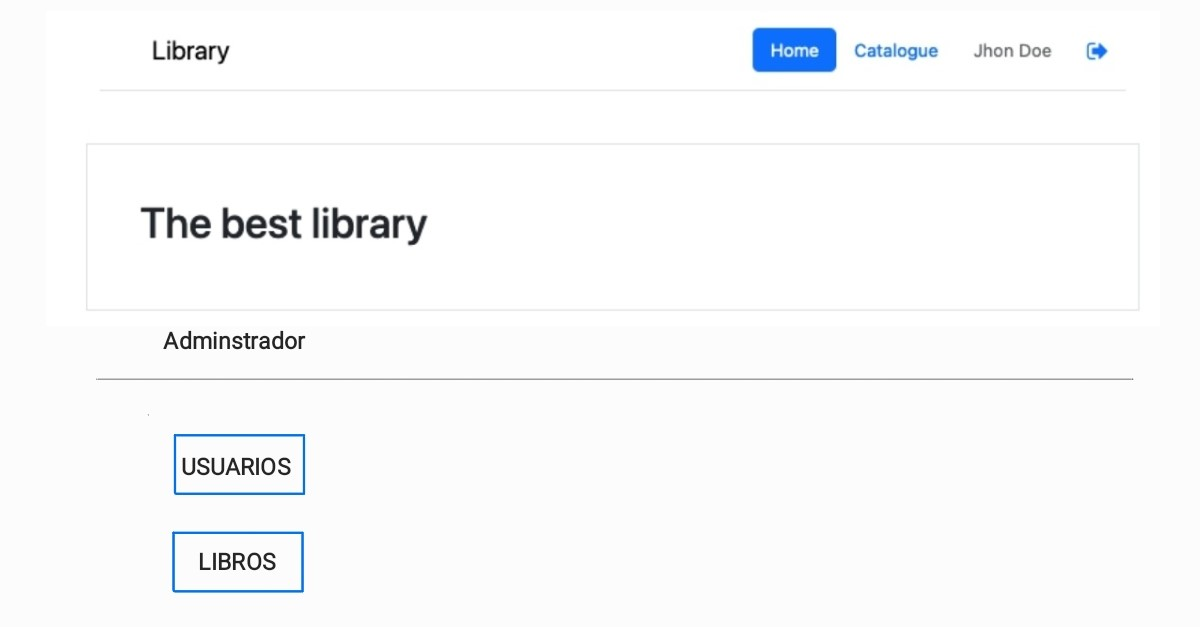
\includegraphics[width=0.8\textwidth]{./img/grafico/MenuAdmin.jpg}
                                \\Figura 3.2.4.2.2: Interfaz del menú de administrador.
                            \end{figure}\\
                            \begin{figure}[H]
                                \centering
                                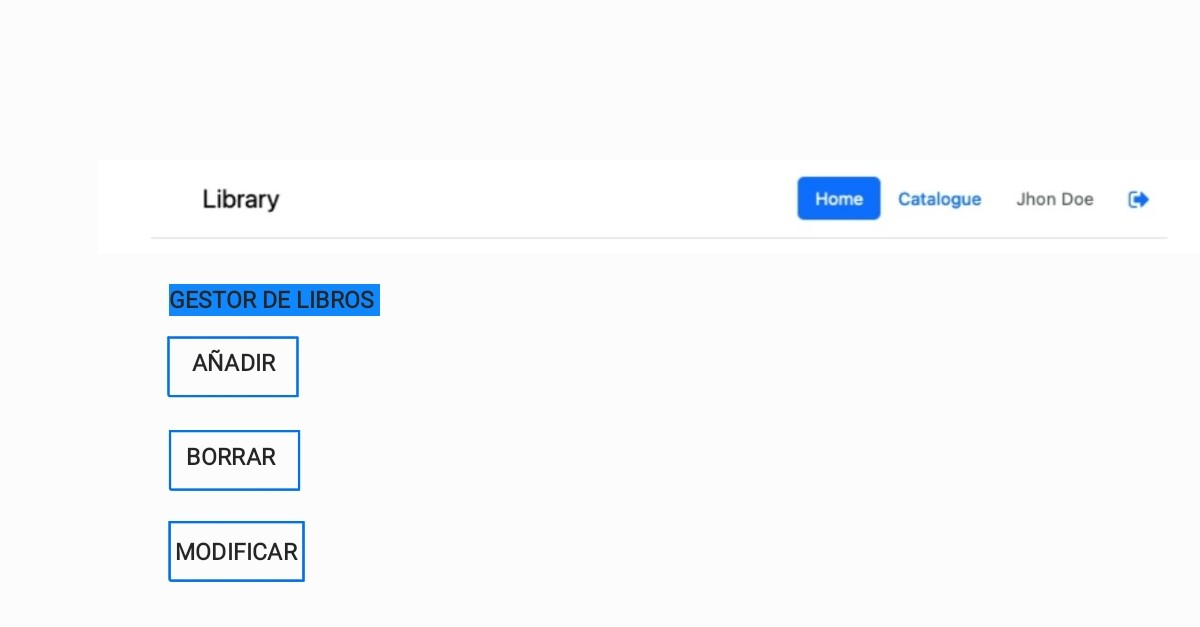
\includegraphics[width=0.8\textwidth]{./img/grafico/MenuGestorLibros.jpg}
                                \\Figura 3.2.4.2.3: Interfaz del menu de gestión de libros.
                            \end{figure}\\
                            \begin{figure}[H]
                                \centering
                                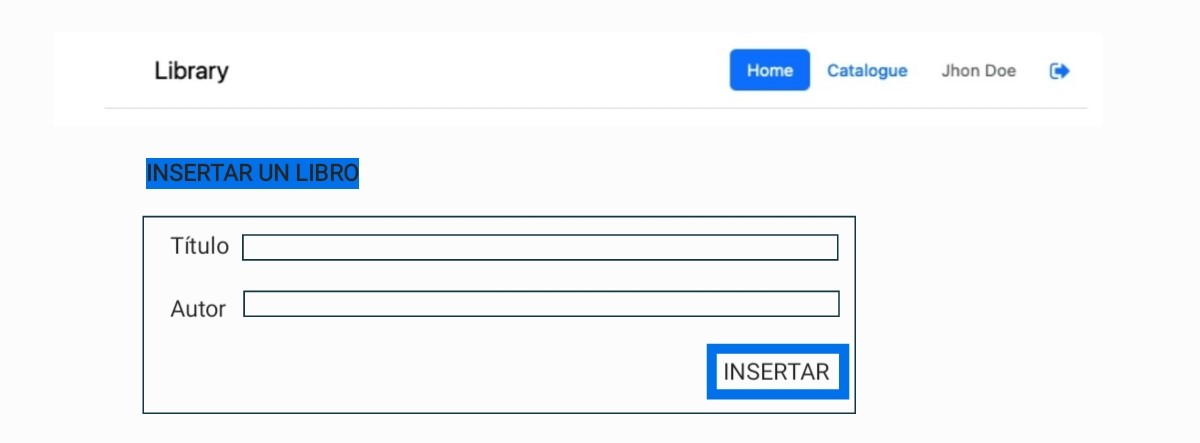
\includegraphics[width=0.8\textwidth]{./img/grafico/InsertarLibro.jpg}
                                \\Figura 3.2.4.2.4: Interfaz para añadir un libro.
                            \end{figure}\\
                            \begin{figure}[H]
                                \centering
                                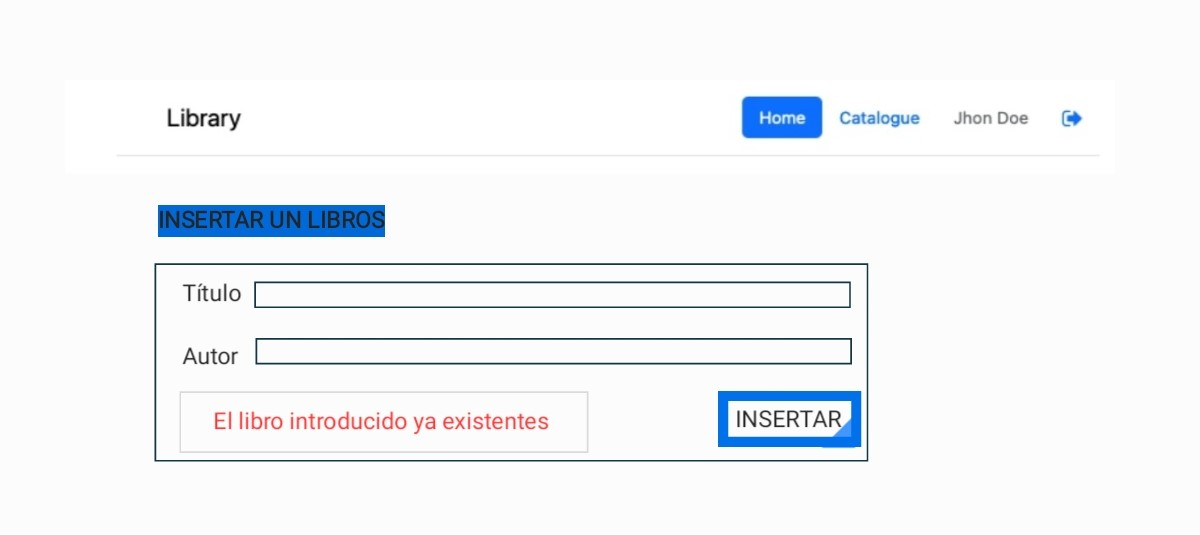
\includegraphics[width=0.8\textwidth]{./img/grafico/ErrorInsertarLibro.jpg}
                                \\Figura 3.2.4.2.5: Interfaz de error al añadir un libro.
                            \end{figure}\\
                            \begin{figure}[H]
                                \centering
                                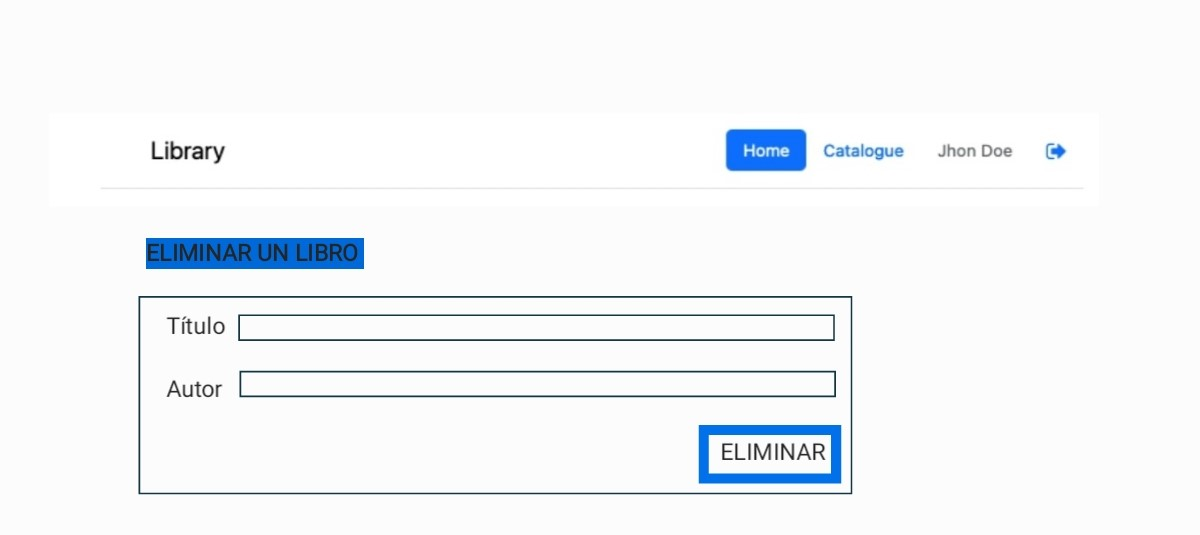
\includegraphics[width=0.8\textwidth]{./img/grafico/EliminarLibro.jpg}
                                \\Figura 3.2.4.2.6: Interfaz para borrar un libro.
                            \end{figure}\\
                            \begin{figure}[H]
                                \centering
                                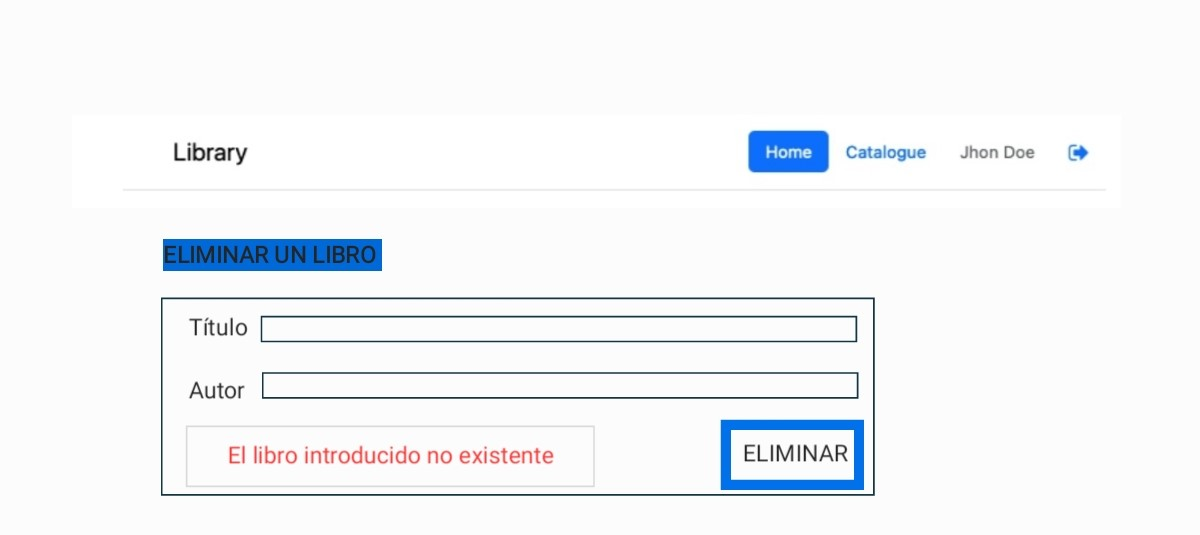
\includegraphics[width=0.8\textwidth]{./img/grafico/ErrorEliminarLibro.jpg}
                                \\Figura 3.2.4.2.7: Interfaz de error al borrar un libro.
                            \end{figure}\\
                            \begin{figure}[H]
                                \centering
                                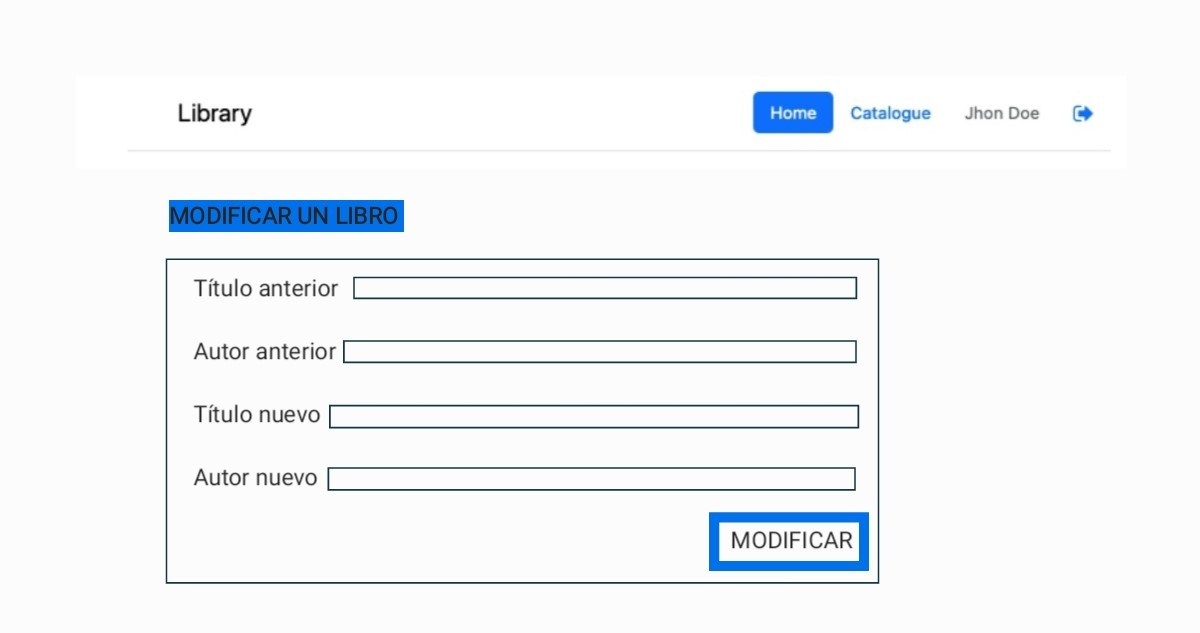
\includegraphics[width=0.8\textwidth]{./img/grafico/ModificarLibro.jpg}
                                \\Figura 3.2.4.2.8: Interfaz para modificar un libro.
                            \end{figure}\\
                            \begin{figure}[H]
                                \centering
                                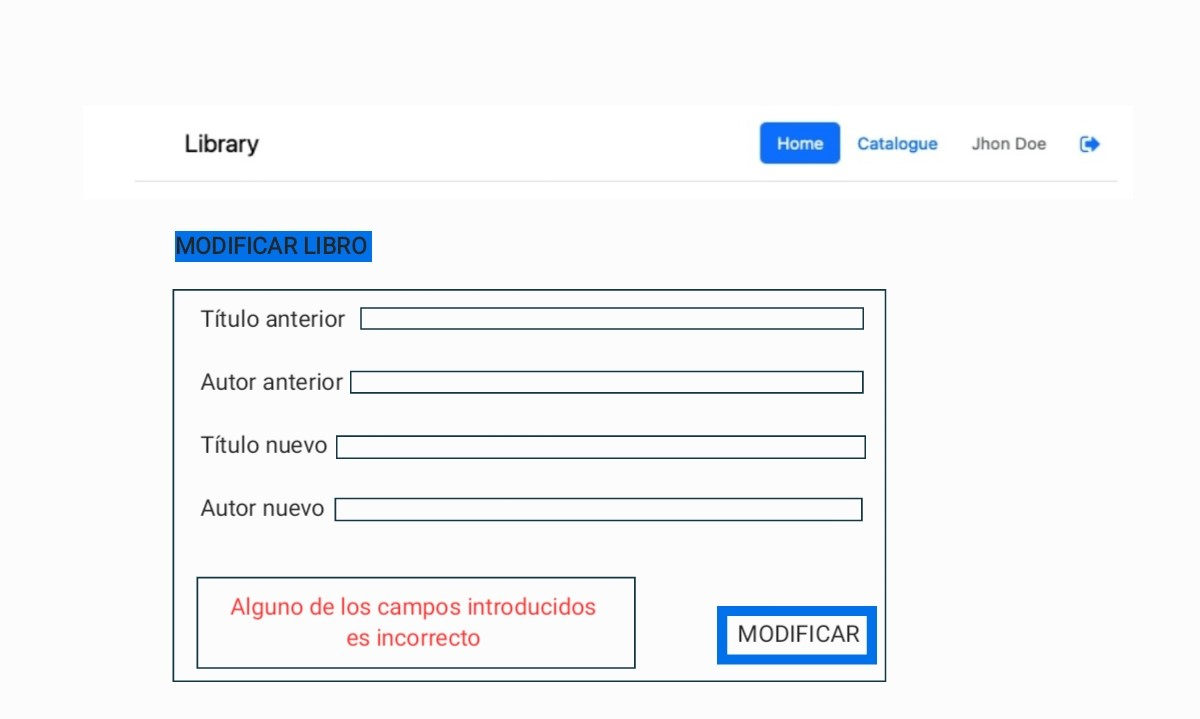
\includegraphics[width=0.8\textwidth]{./img/grafico/ErrorModificarLibro.jpg}
                                \\Figura 3.2.4.2.9: Interfaz de error al modificar un libro.
                            \end{figure}\\
                            \hline
                        \end{longtable}
                    \end{center}
                    \clearpage
            \subsection{Foros}
                \begin{center}
                    \begin{longtable}{|p{\linewidth}|}
                        \hline
                        \textbf{Responsable:} Ainhize Martinez\\
                        \hline
                        \begin{figure}[H]
                            \centering
                            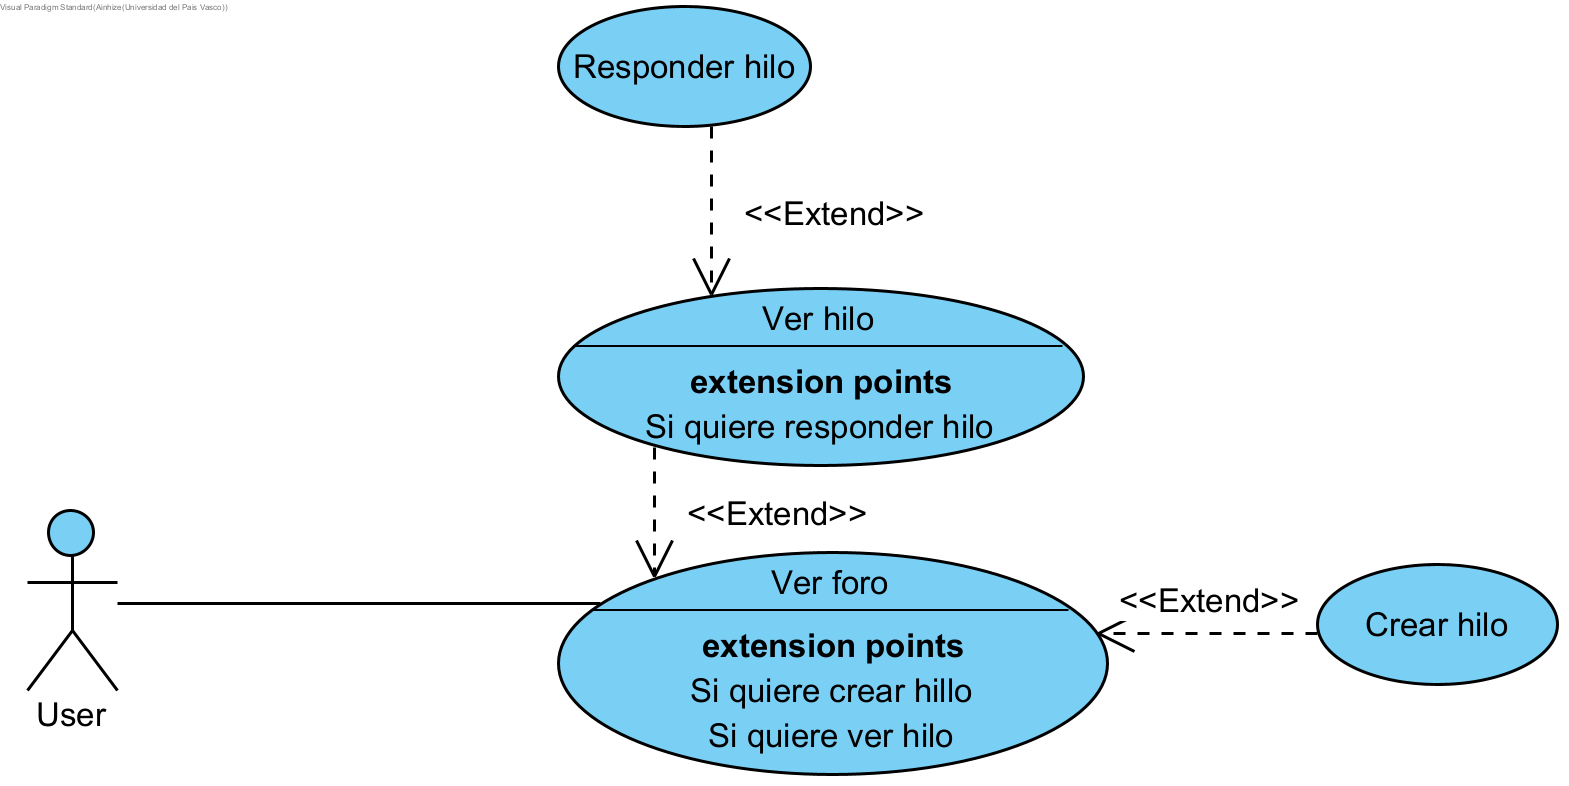
\includegraphics[width=0.8\textwidth]{./img/casos_uso/CasoForo.png}
                            \\Figura 3.2.5.1: Diagrama de casos de uso de la subfuncionalidad de foros
                        \end{figure}\\
                        \hline
                        \textbf{Nombre:} Ver Foros\\
                        \hline
                        \textbf{Descripción:} Permite al usuario acceder al foro, crear hilos nuevos, explorar todos los hilos, además de contestar hilos.\\
                        \hline
                        \textbf{Actores:} Usuario\\
                        \hline
                        \textbf{Precondiciones:} Estar identificado en el sistema.\\
                        \hline
                        \textbf{Requisitos no funcionales:} Ninguno\\
                        \hline
                        \textbf{Flujo de Eventos:}
                        \begin{enumerate}
                            \item El usuario selecciona 'Foro' para acceder a él.
                            \begin{enumerate}
                                \item Se le muestra toda la lista de hilos. [Figura 3.2.5.2]
                                \begin{enumerate}
                                    \item Si el usuario pulsa en '+Hilo' se le abre una ventana para crear un hilo nuevo. [Figura 3.2.5.3]
                                    \item Si el usuario selecciona un hilo se le mostraran las respuesta al hilo. [Figura 3.2.5.4]
                                    \begin{enumerate}
                                        \item Si el usuario pulsa en '+Mensaje' se le abre una ventana para responder al hilo [Figura 3.2.5.5]
                                    \end{enumerate}
                                \end{enumerate}
                            \end{enumerate}
                        \end{enumerate}\\
                        \hline
                        \textbf{Poscondiciones:} Ninguna\\
                        \hline
                        \textbf{Interfaz Gráfica:}\\
                        \begin{figure}[H]
                            \centering
                            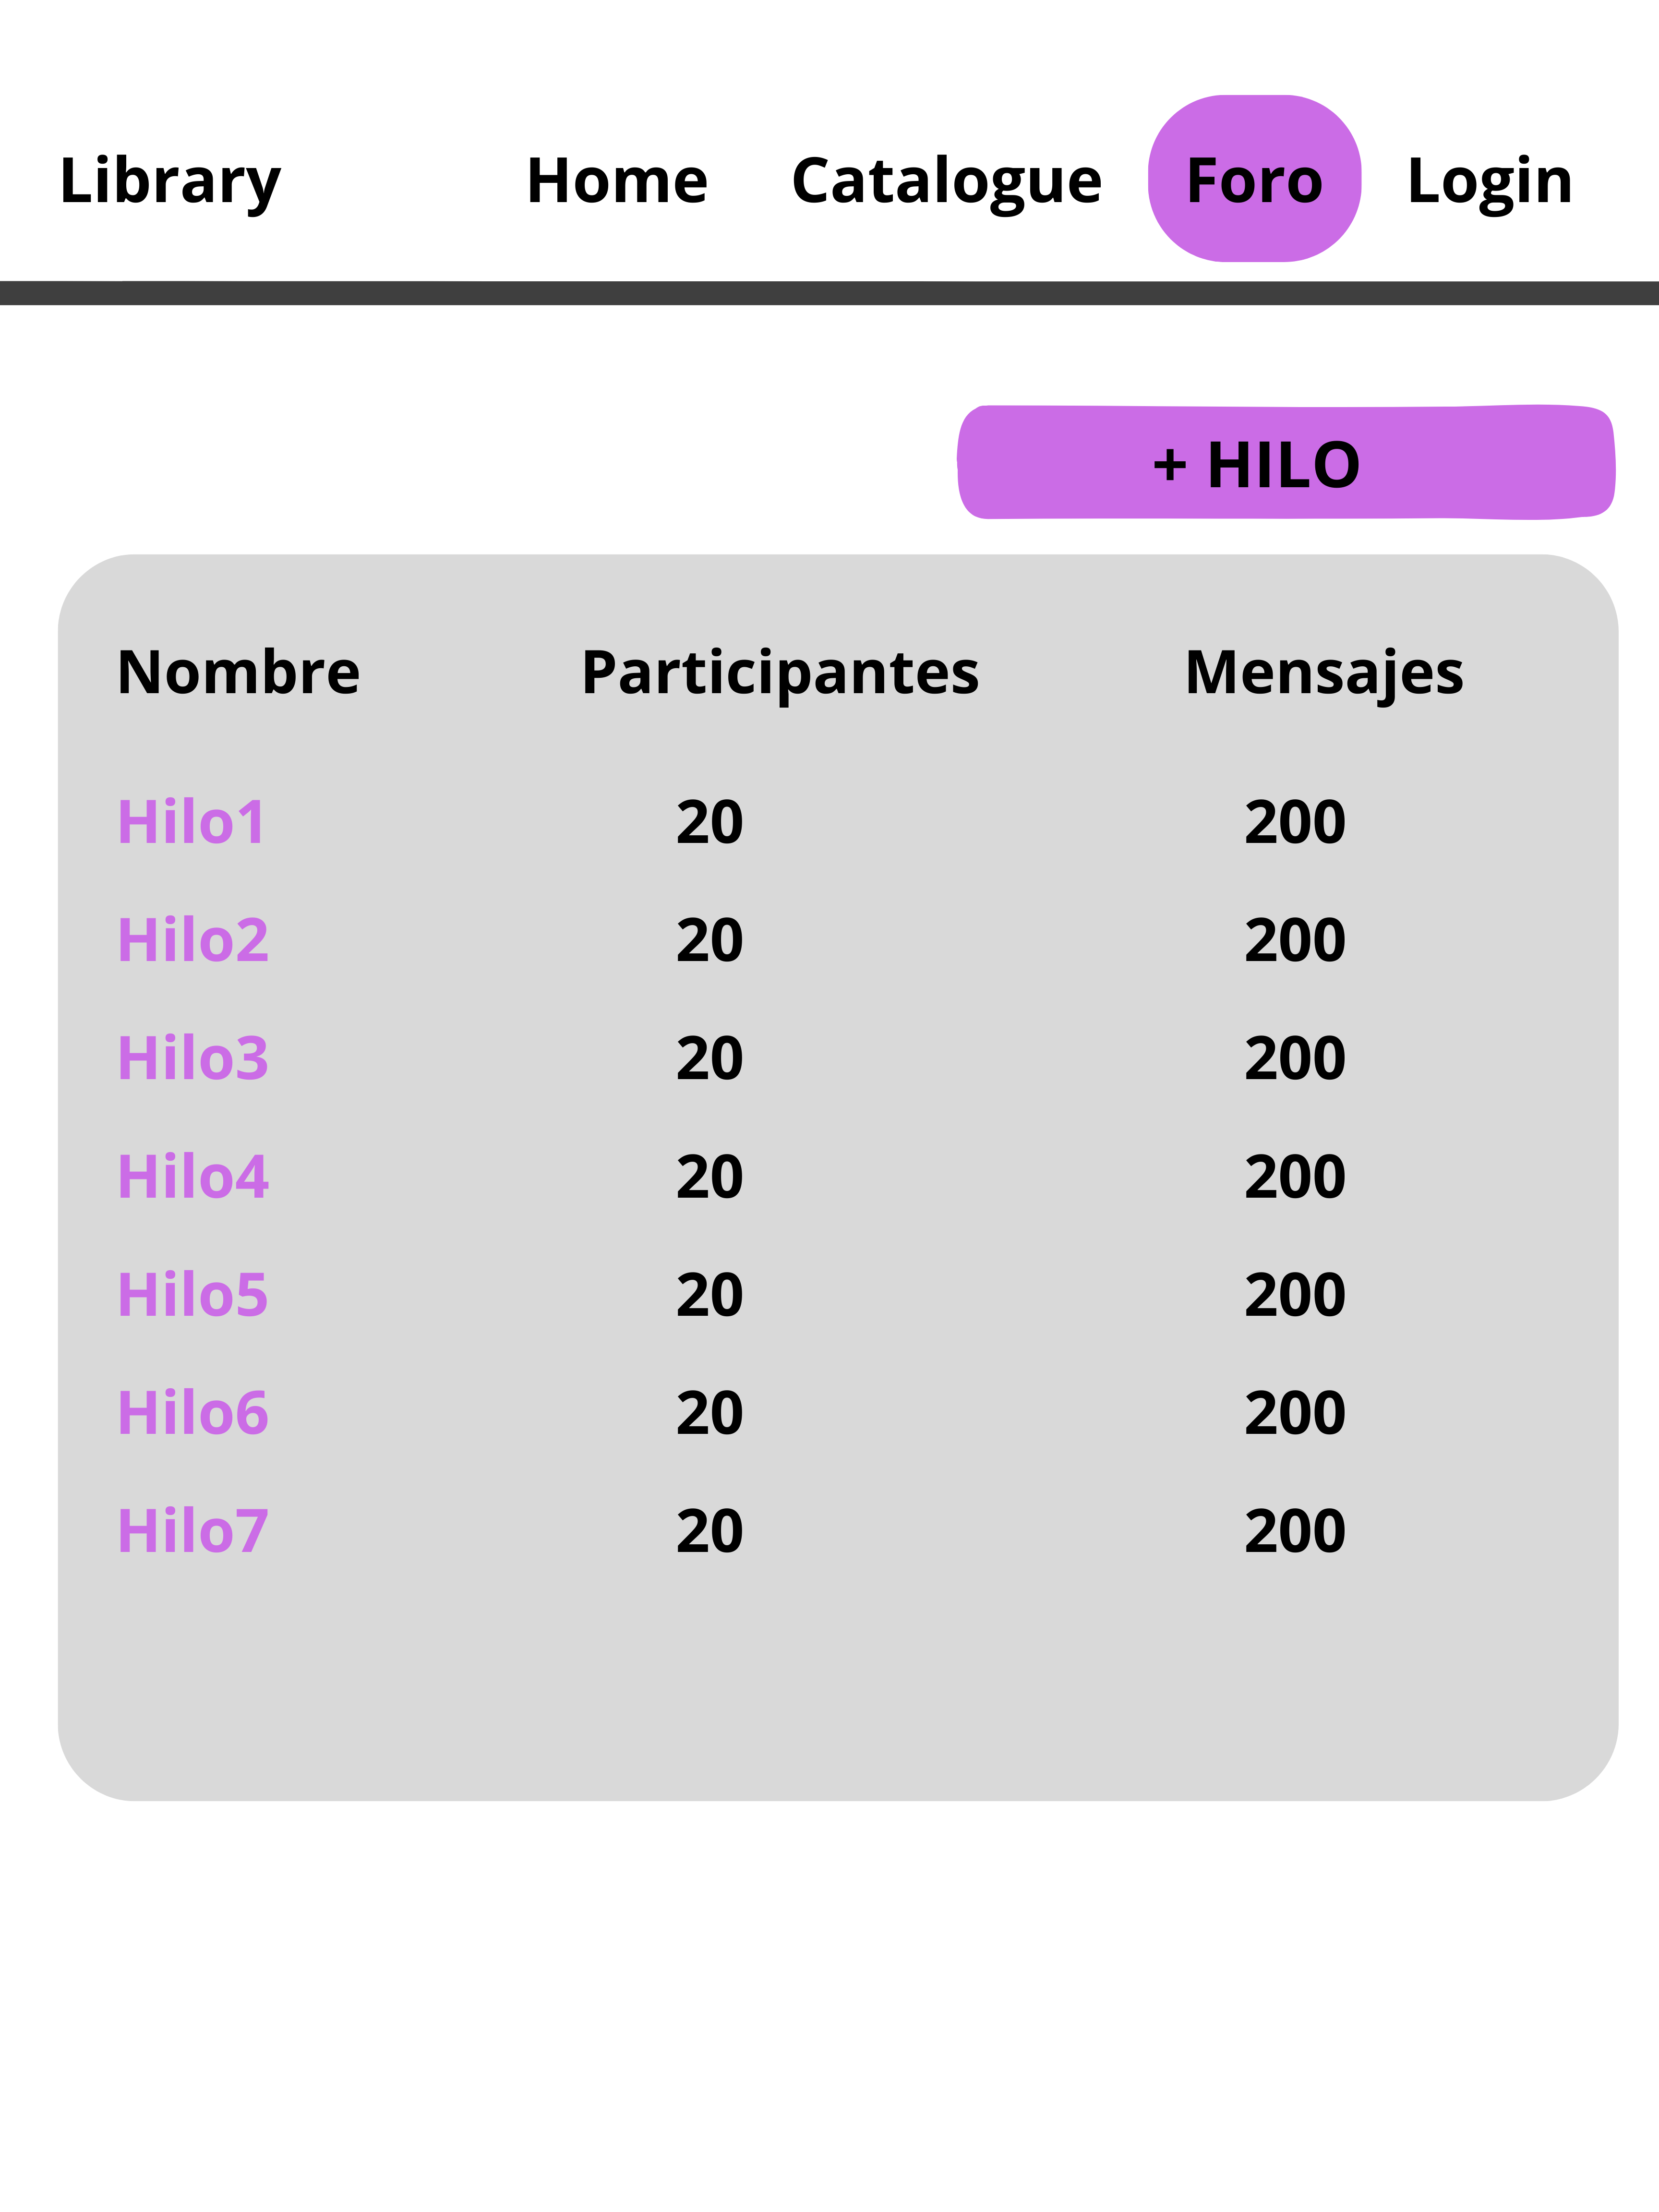
\includegraphics[width=0.8\textwidth]{./img/grafico/Foro.png}
                            \\Figura 3.2.5.2: Interfaz del foro.
                        \end{figure}\\
                        \begin{figure}[H]
                            \centering
                            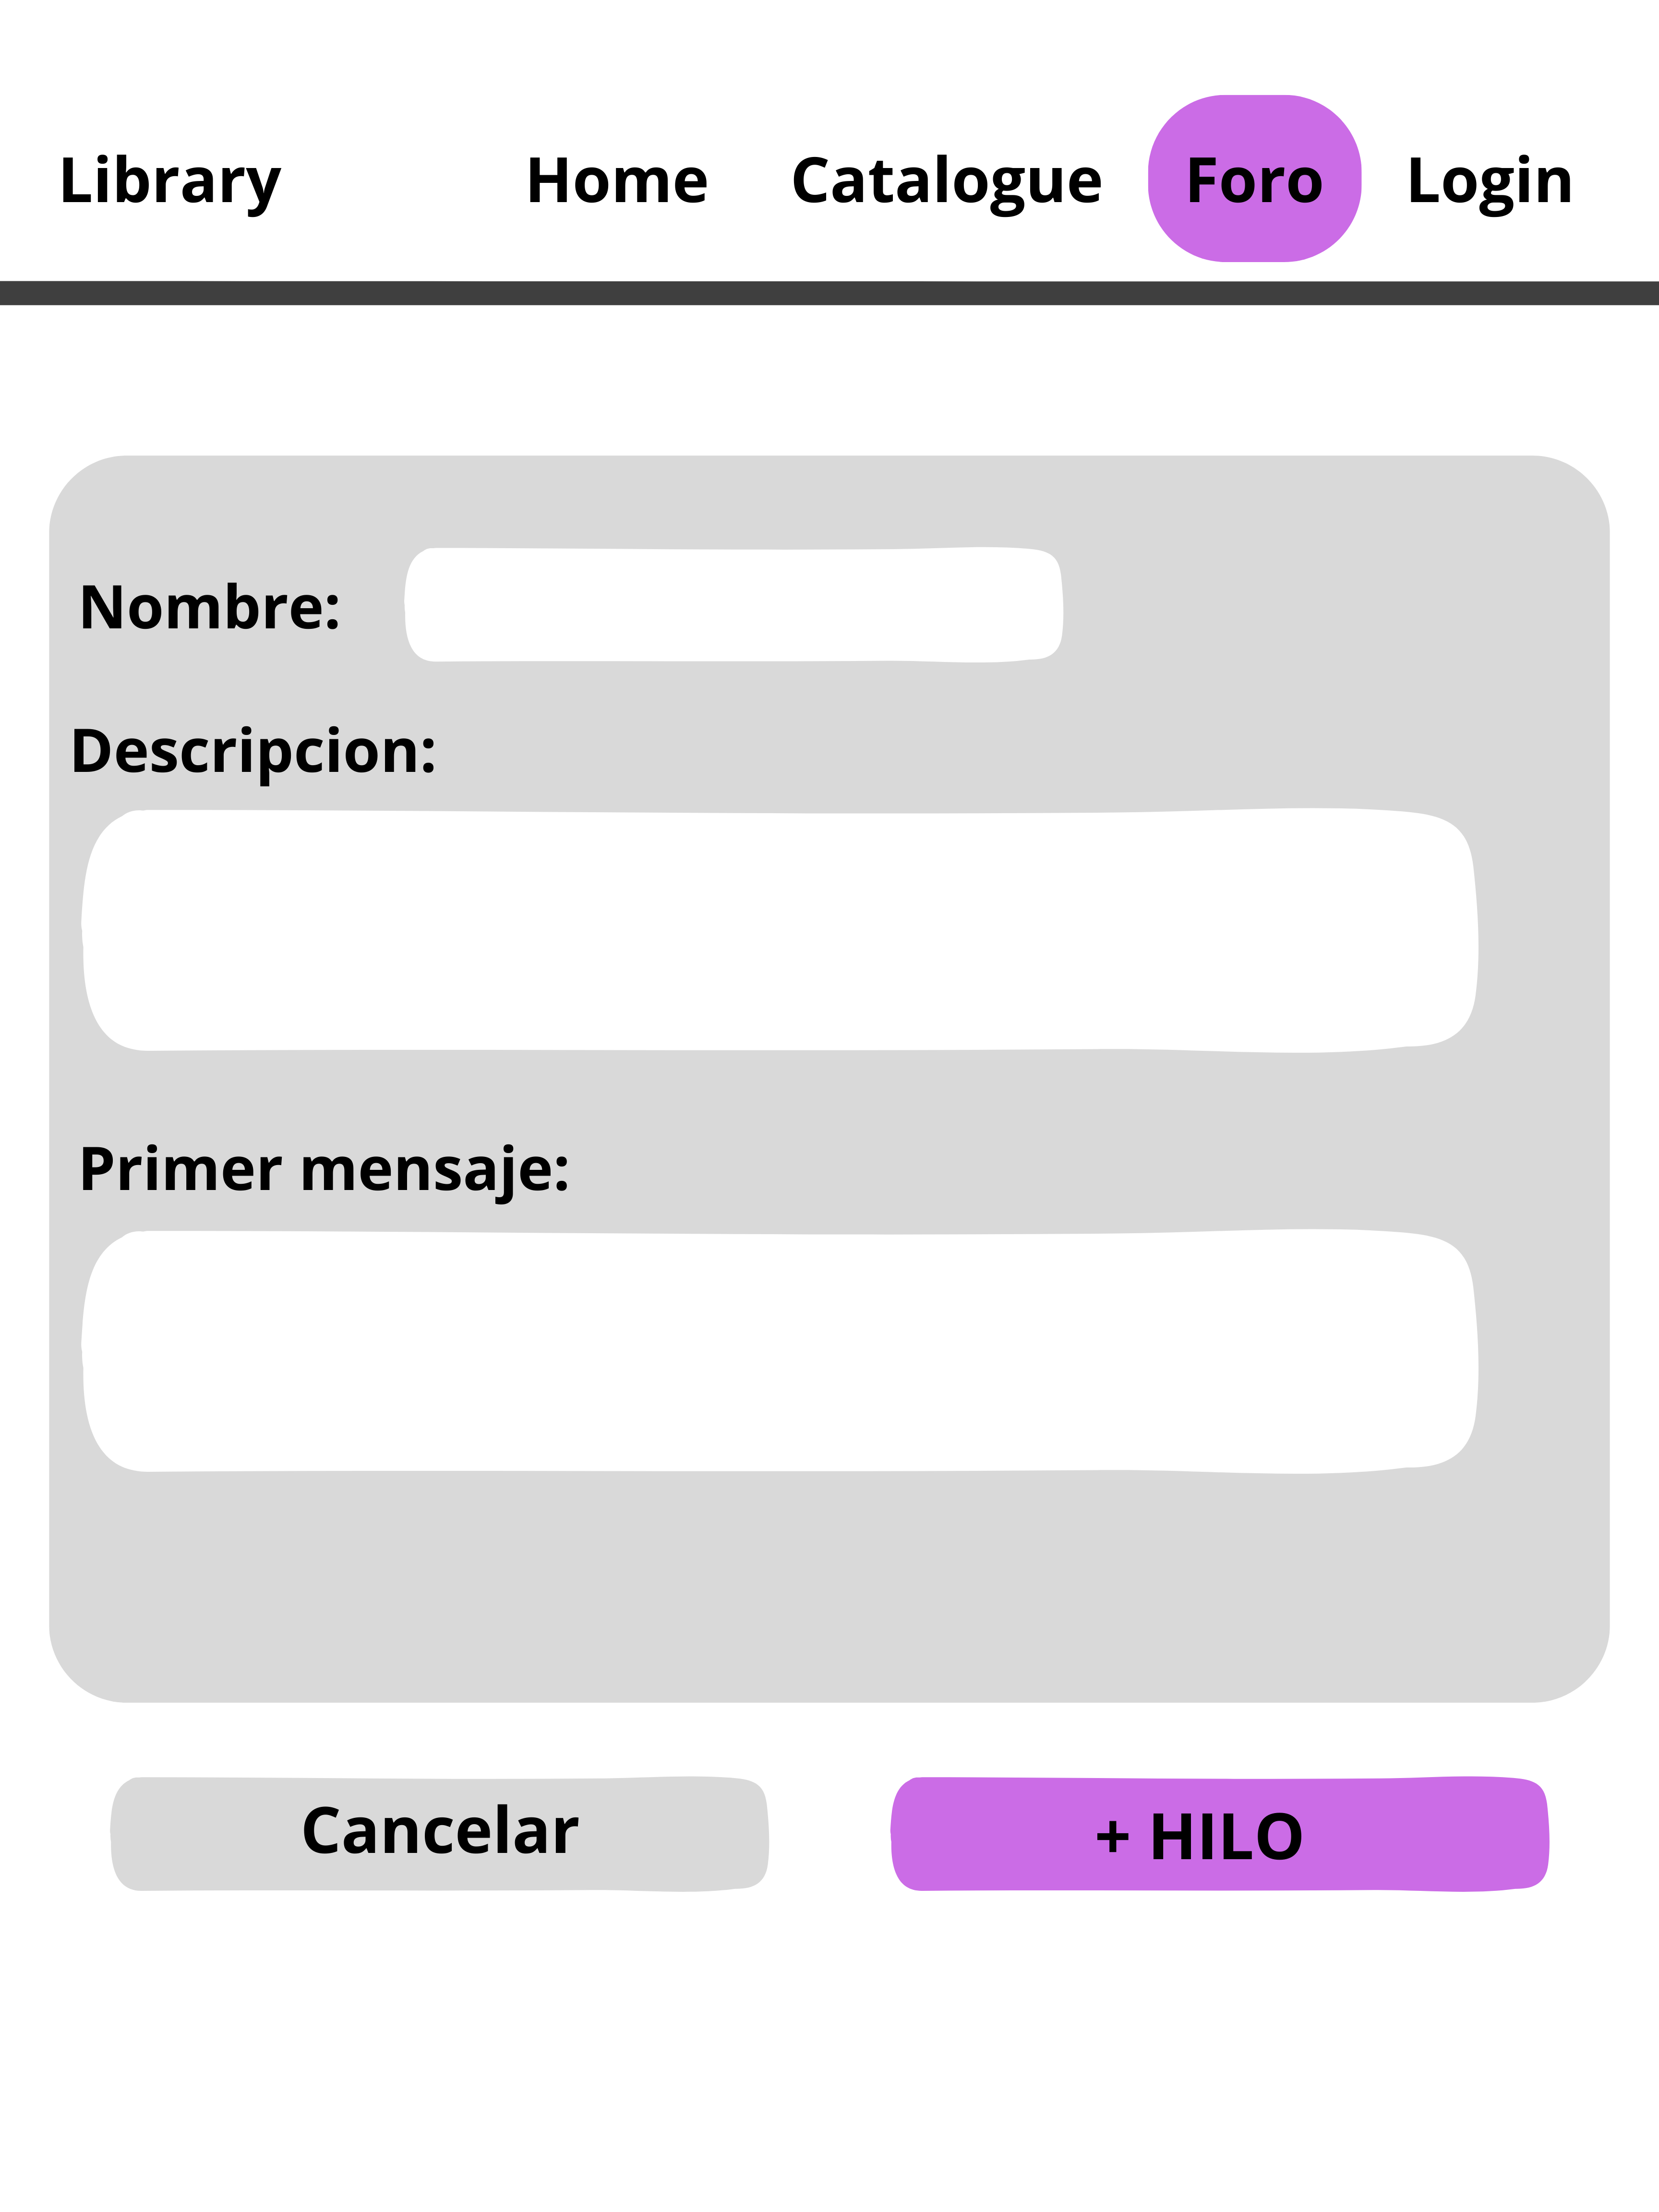
\includegraphics[width=0.8\textwidth]{./img/grafico/Foro2.png}
                            \\Figura 3.2.5.3: Interfaz para crear un hilo del foro.
                        \end{figure}\\
                        \begin{figure}[H]
                            \centering
                            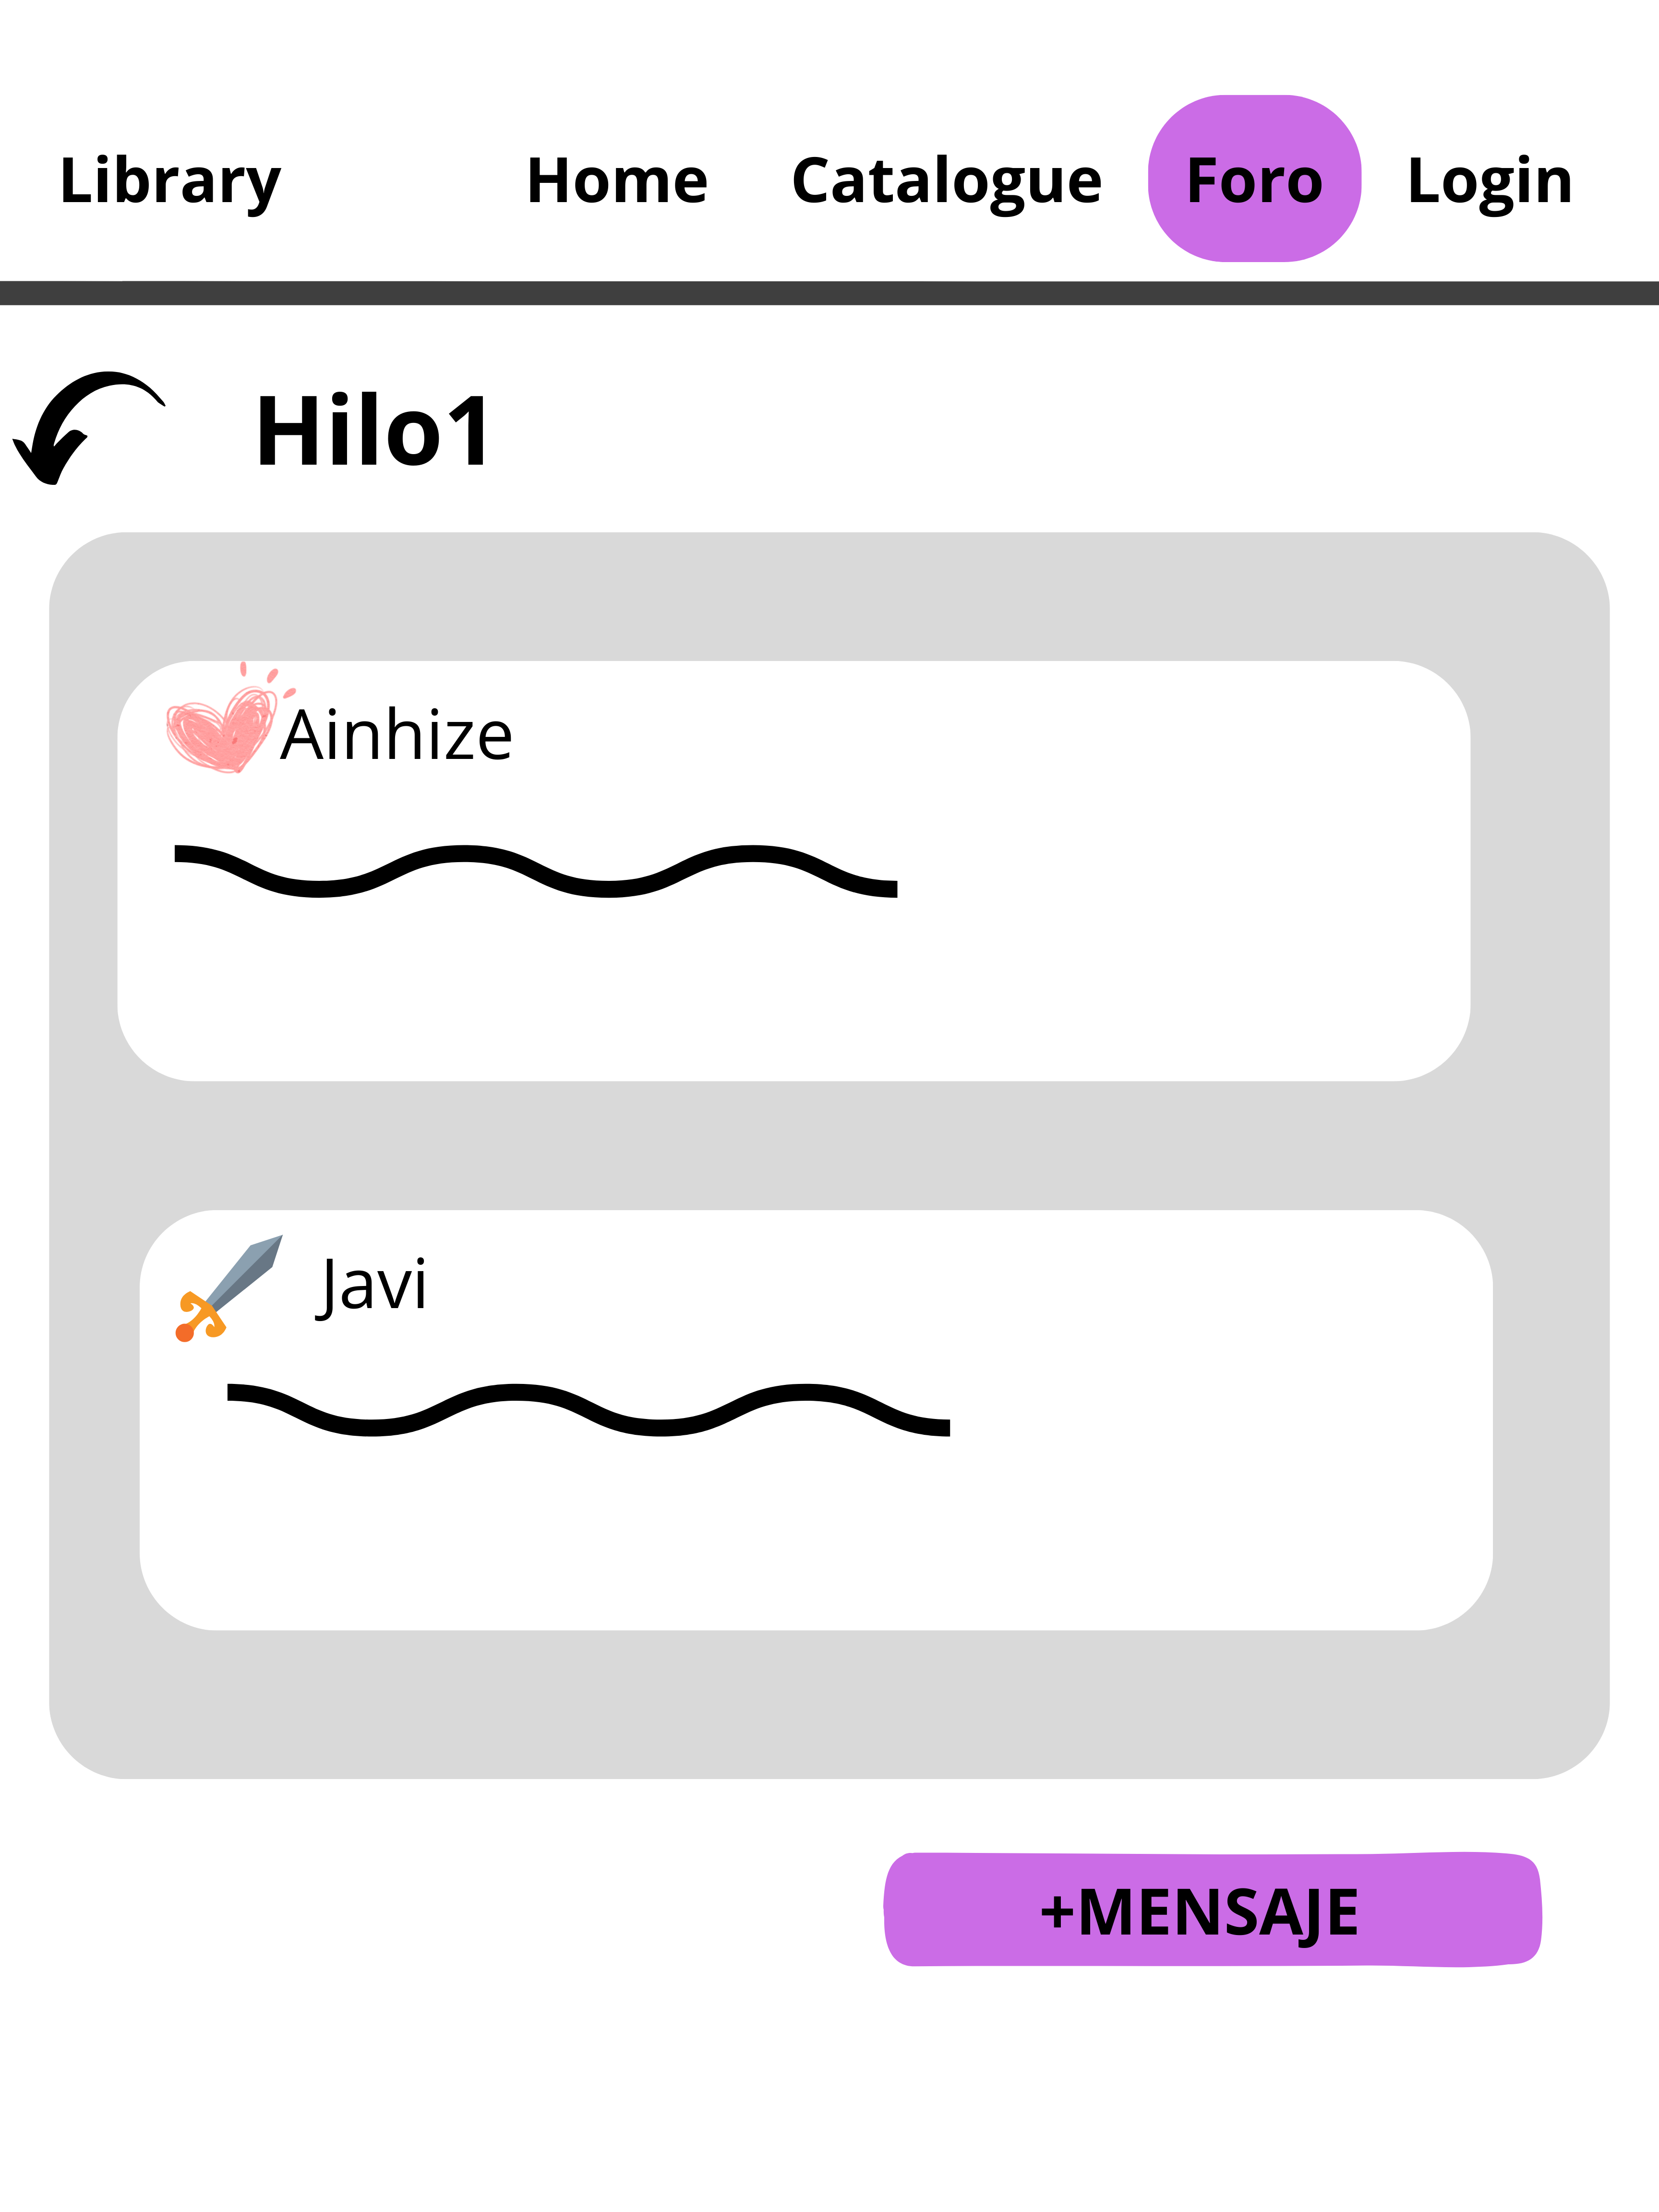
\includegraphics[width=0.8\textwidth]{./img/grafico/Foro3.png}
                            \\Figura 3.2.5.4: Interfaz para ver un hilo del foro.
                        \end{figure}\\
                        \begin{figure}[H]
                            \centering
                            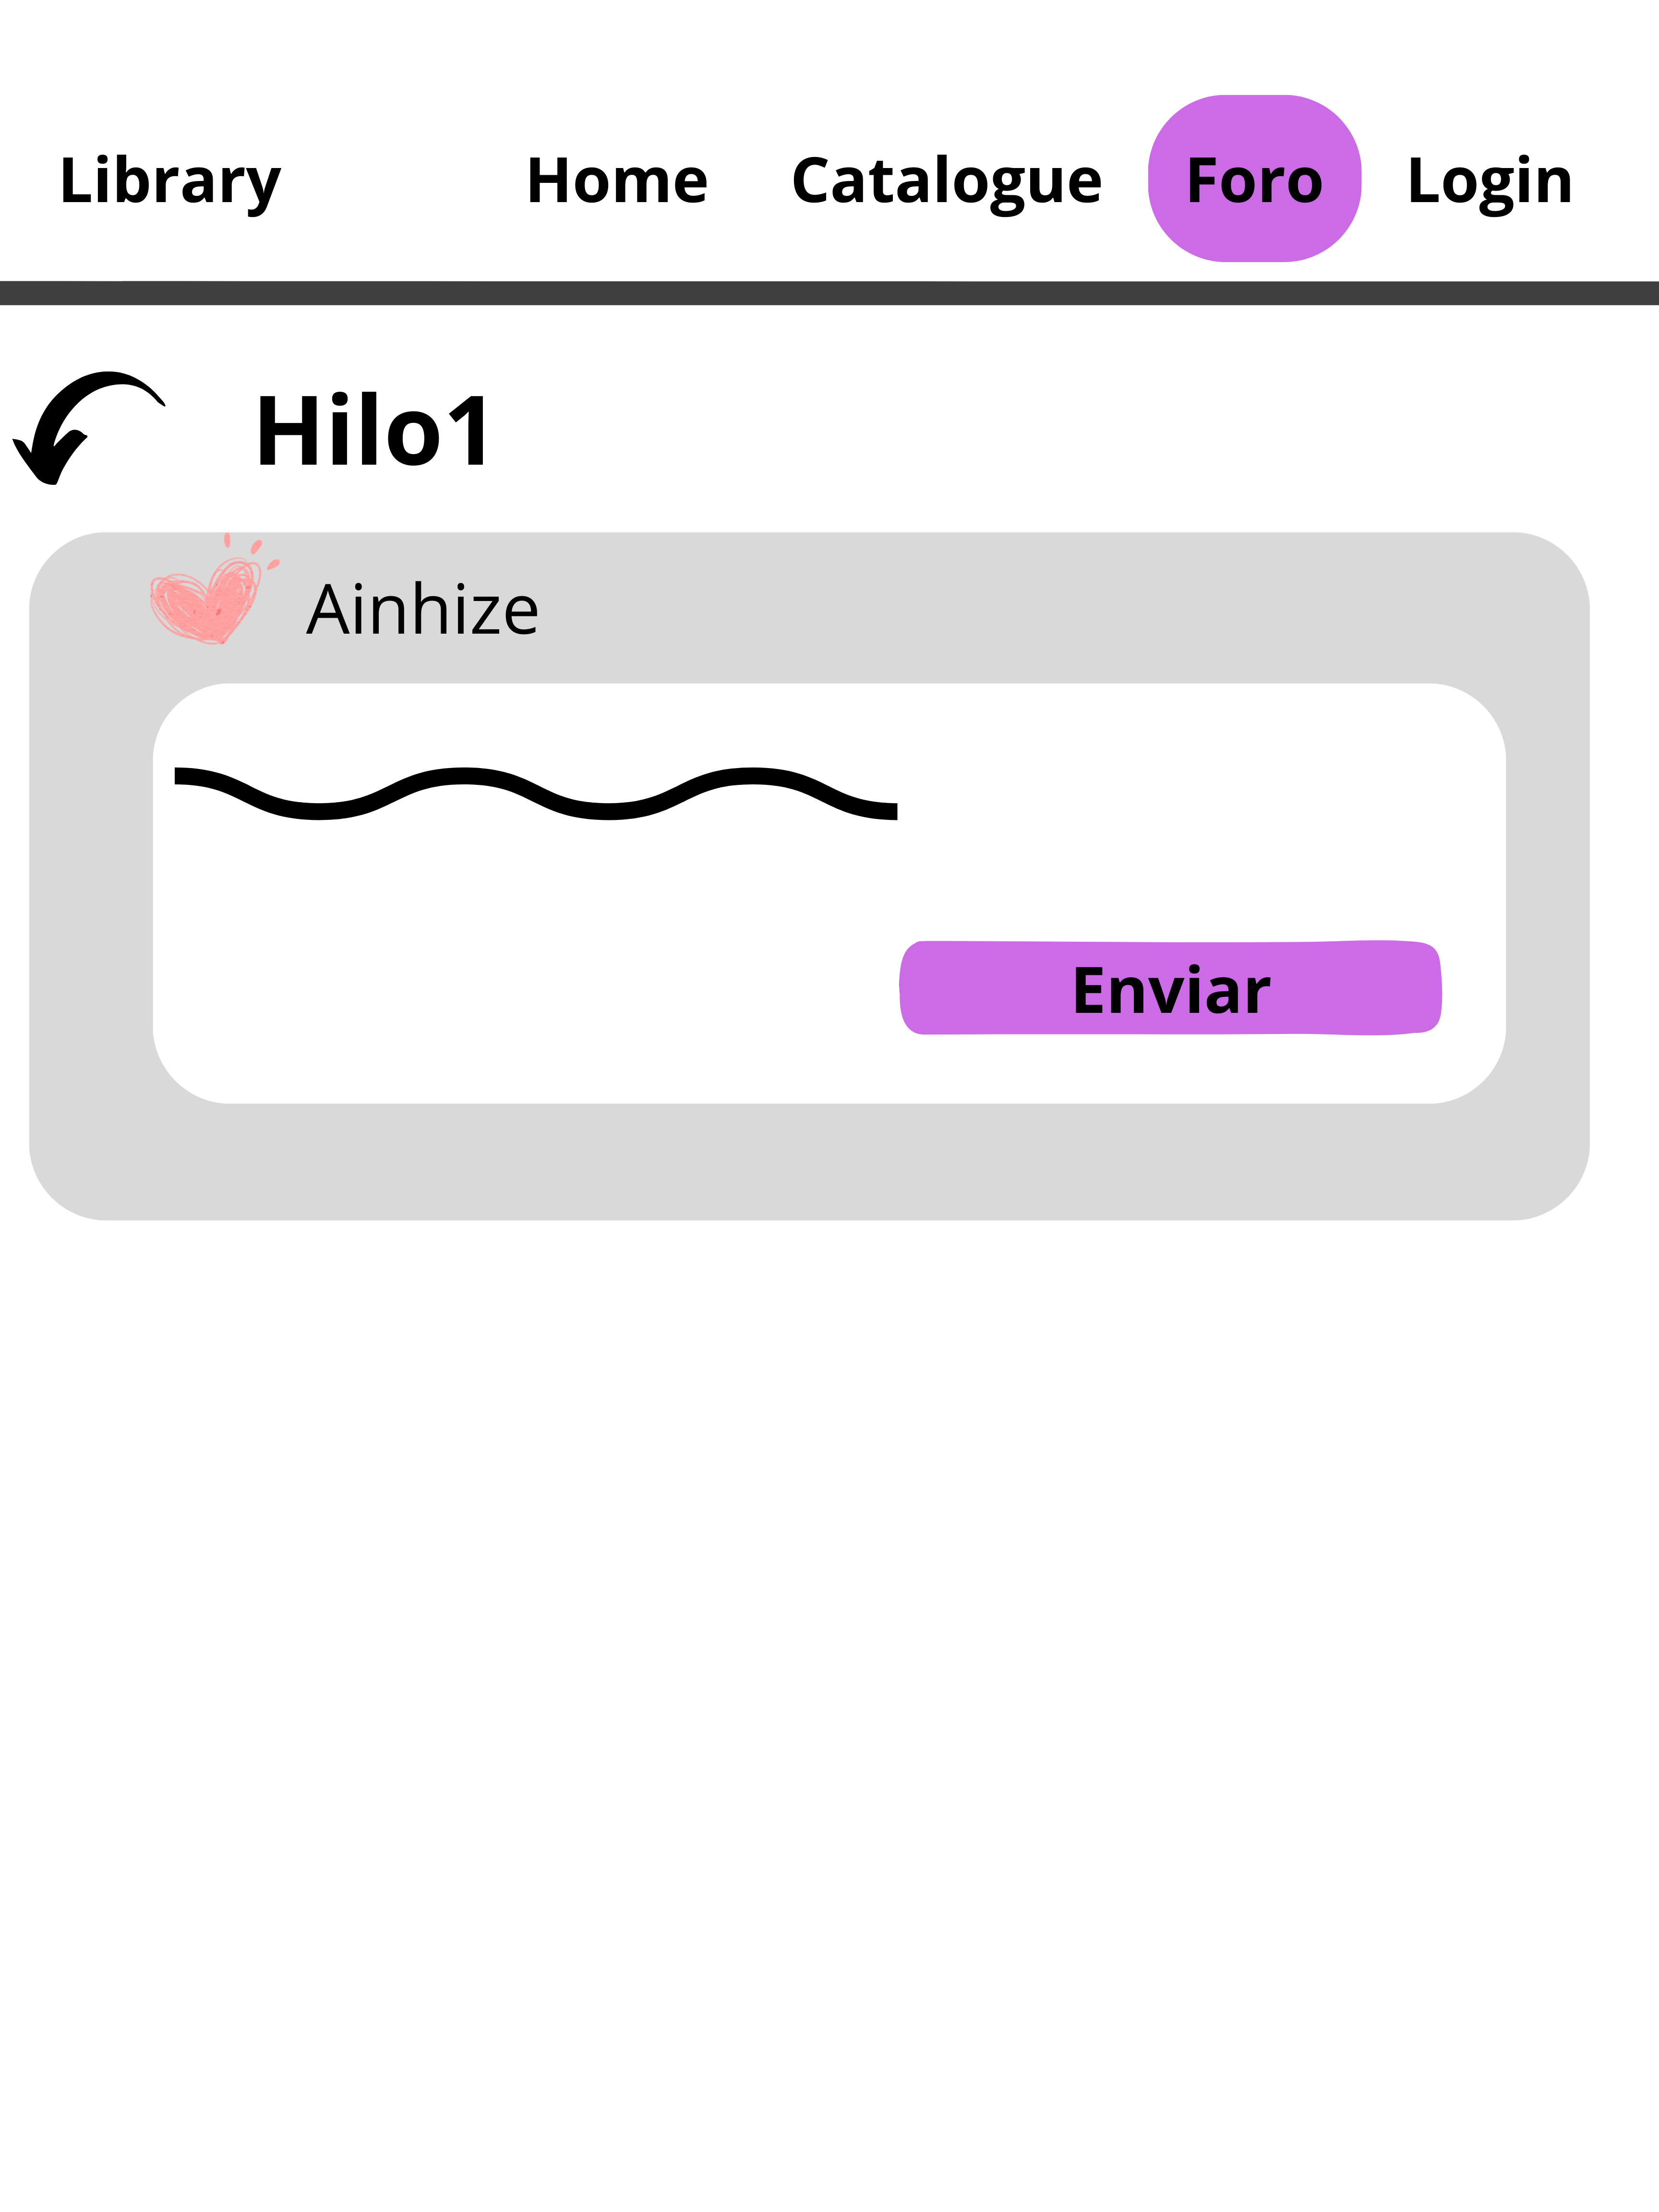
\includegraphics[width=0.8\textwidth]{./img/grafico/Foro4.png}
                            \\Figura 3.2.5.5: Interfaz para responder a un hilo.
                        \end{figure}\\
                        \hline
                    \end{longtable}
                \end{center}
                \clearpage
            \subsection{Recomendaciones del sistema}
                \begin{center}
                    \begin{longtable}{|p{\linewidth}|}
                        \hline
                        \textbf{Responsable:} Xabier Gabiña\\
                        \hline
                        \begin{figure}[H]
                            \centering
                            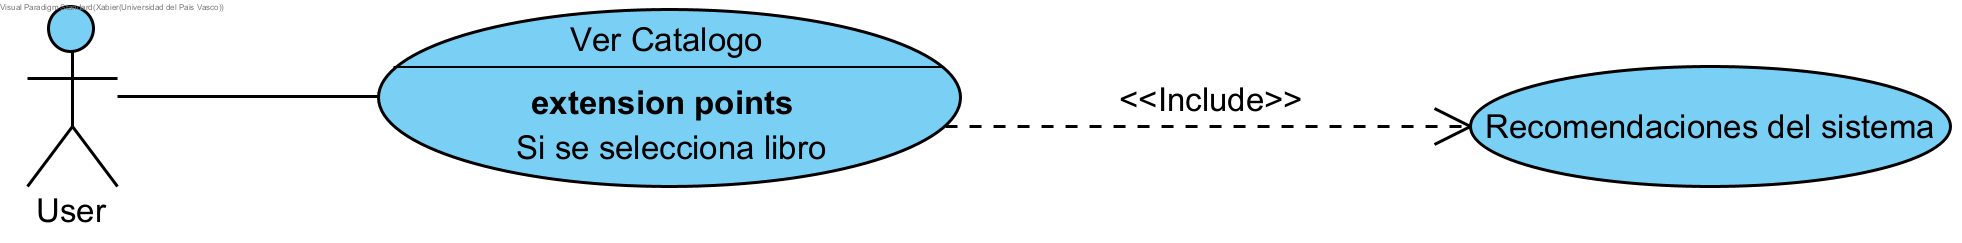
\includegraphics[width=0.8\textwidth]{./img/casos_uso/RecomendacionesLibros.png}
                            \\Figura 3.2.6.1: Diagrama de casos de uso de la subfuncionalidad de recomendaciones de libros
                        \end{figure}\\
                        \hline
                        \textbf{Nombre:} Recomendaciones del sistema\\
                        \hline
                        \textbf{Descripción:} Muestra una lista en la parte superior del catálogo mostrando los libros con más préstamos del sistema en funcion de los gustos del usuario.\\
                        \hline
                        \textbf{Actores:} Usuario\\
                        \hline
                        \textbf{Precondiciones:} Estar identificado en el sistema y haber tenido un libro reservado\\
                        \hline
                        \textbf{Requisitos no funcionales:} Ninguno\\
                        \hline
                        \textbf{Flujo de Eventos:}
                        \begin{enumerate}
                            \item El usuario entra en el catalogo para ver los libros disponibles.
                            \begin{enumerate}
                                \item Se le muestra en la parte superior de la pantalla una serie de libros basadas en los generos y peliculas que consume el usuario. [Figura 3.2.6.2]
                            \end{enumerate}
                        \end{enumerate}\\
                        \hline
                        \textbf{Poscondiciones:} Ninguna\\
                        \hline
                        \textbf{Interfaz Gráfica:}\\
                        \begin{figure}[H]
                            \centering
                            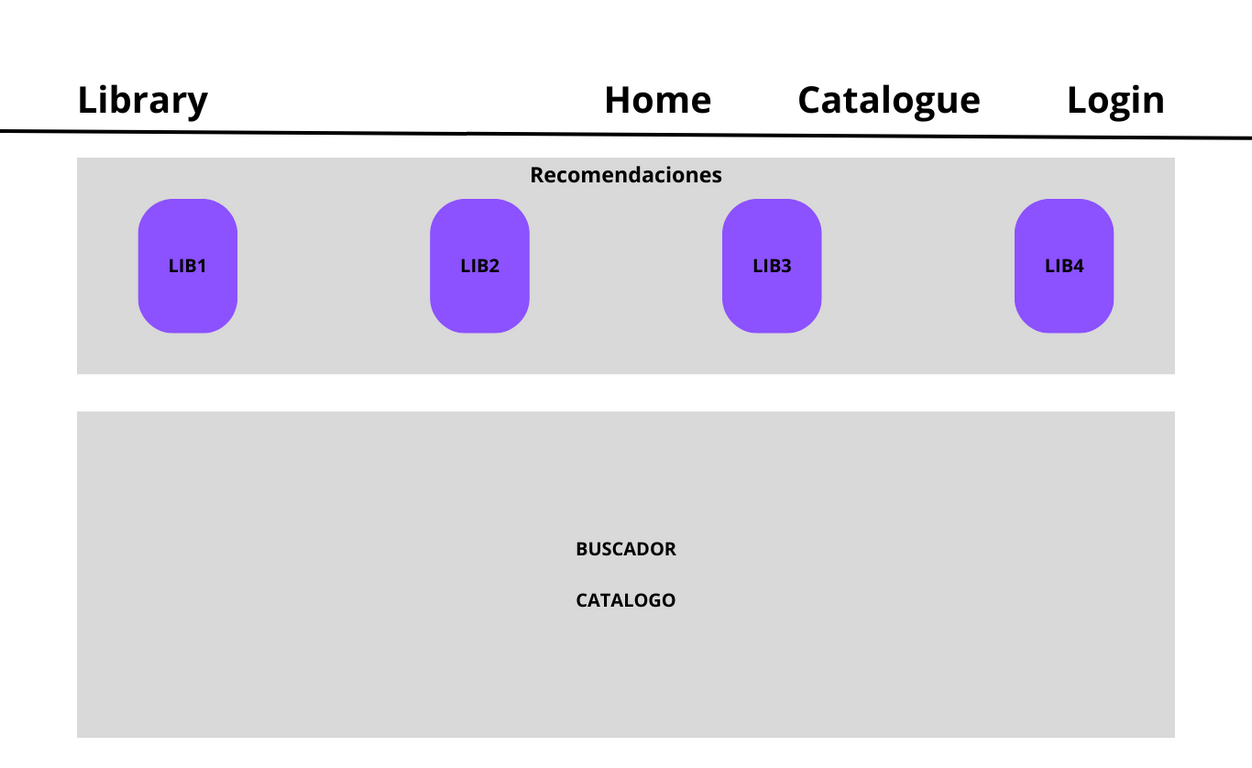
\includegraphics[width=0.8\textwidth]{./img/grafico/recom_lib.png}
                            \\Figura 3.2.6.2: Interfaz de recomendaciones de libros.
                        \end{figure}\\
                        \hline
                    \end{longtable}
                \end{center}
                \clearpage
            \subsection{Recomendaciones de amigos}
                \begin{center}
                    \begin{longtable}{|p{\linewidth}|}
                        \hline
                        \textbf{Responsable:} Kepa Reche\\
                        \hline
                        \begin{figure}[H]
                            \centering
                            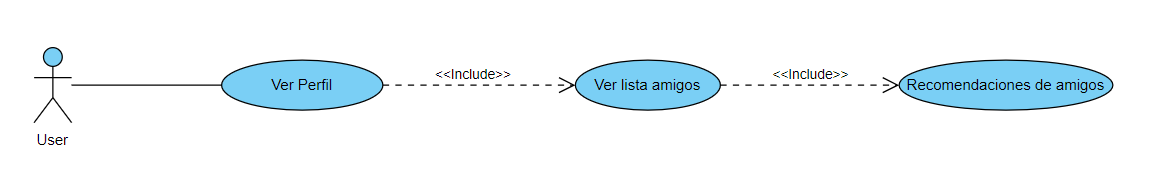
\includegraphics[width=0.8\textwidth]{./img/casos_uso/RecomendacionesAmigos.png}
                            \\Figura 3.2.7.1: Diagrama de casos de uso de la subfuncionalidad de recomendaciones de amigos
                        \end{figure}\\
                        \hline
                        \textbf{Nombre:} Ver amigos recomendados\\
                        \hline
                        \textbf{Descripción:} Muestra una lista en la parte superior de la lista de amigos mostrando posibles nuevos amigos basados en amigos de tus amigos o personas con las que tengas lecturas relacionadas.\\
                        \hline
                        \textbf{Actores:} Usuario\\
                        \hline
                        \textbf{Precondiciones:} Estar identificado en el sistema y tener algun amigo o libro guardado en tu perfil\\
                        \hline
                        \textbf{Requisitos no funcionales:} Ninguno\\
                        \hline
                        \textbf{Flujo de Eventos:}
                        \begin{enumerate}
                            \item El Usuario entra en su perfil.
                            \begin{enumerate}
                                \item Se le muestra en la parte superior de la lista de amigos varias personas recomendadas segun las lecturas en comun y amigos de amigos. [Figura 3.2.7.2]
                            \end{enumerate}
                        \end{enumerate}\\
                        \hline
                        \textbf{Poscondiciones:} Ninguna\\
                        \hline
                        \textbf{Interfaz Gráfica:}\\
                        \begin{figure}[H]
                            \centering
                            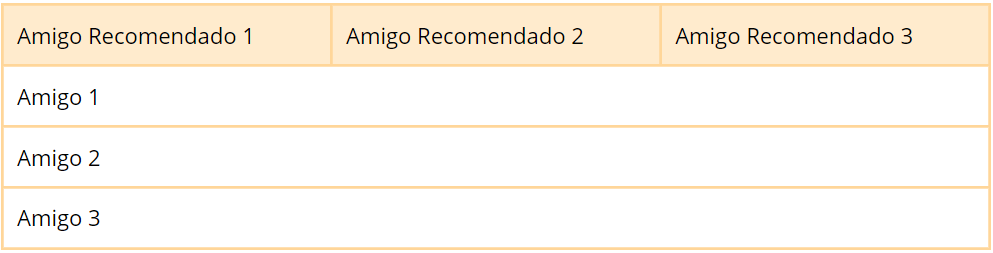
\includegraphics[width=0.8\textwidth]{./img/grafico/IU Recomendaciones de amigos.PNG}
                            \\Figura 3.2.7.2: Interfaz de recomendaciones de amigos.
                        \end{figure}\\
                        \hline
                    \end{longtable}
                \end{center}
                \clearpage
    \chapter{Modelo de Dominio}
        \section{Diagrama de modelo de dominio}
            \begin{figure}[H]
                \centering
                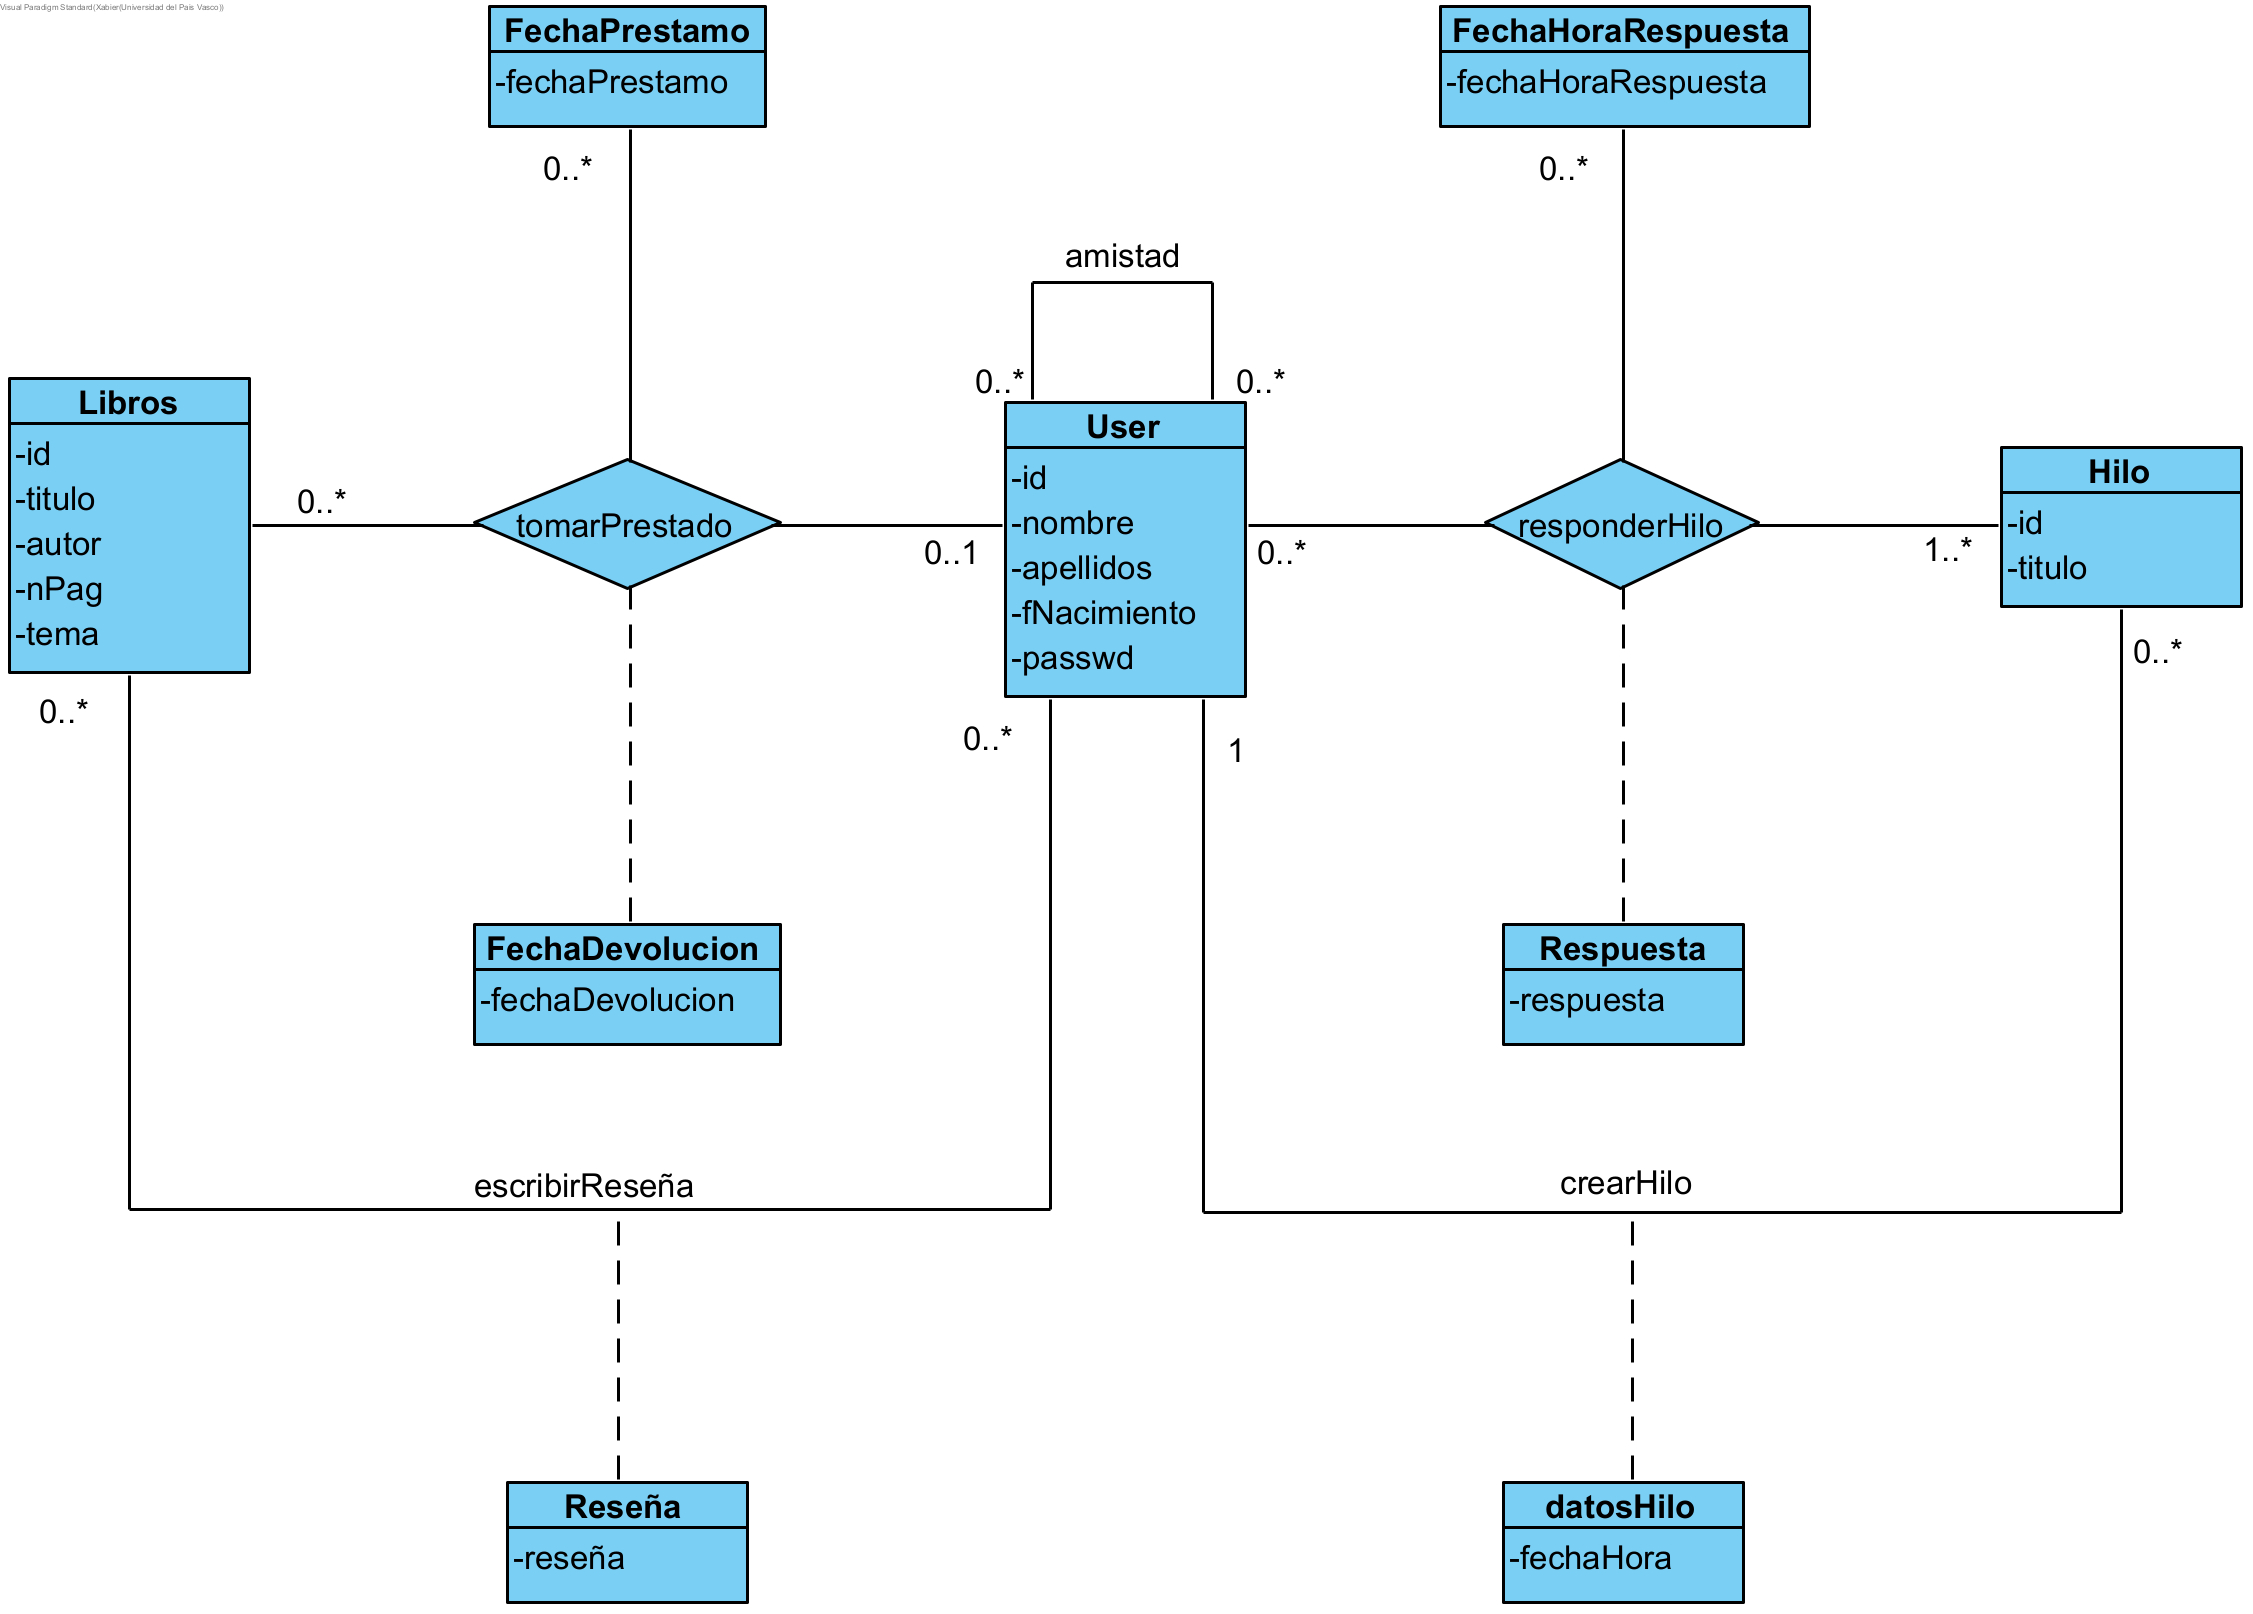
\includegraphics[width=1.0\textwidth]{img/dominio/Dominio.png}
                \caption{Diagrama de modelo de dominio}
            \end{figure}
        \clearpage
        \section{Desarrollo del modelo de dominio}
            \subsection{Entitades}
                \subsubsection{User}
                    La entidad usuario representa a los usuarios de la aplicacion. Dentro almacena sus datos personales como su id, nombre, apellidos, fecha de nacimiento...
                \subsubsection{Admin}
                    La entidad admin representa a los administradores de la aplicacion. Dentro almacena su id, nombre, apellidos y su contraseña.
                \subsubsection{Libros}
                    La entidad libro representa a los libros de la aplicacion. Dentro almacena sus datos como su id, titulo, autor, numero de paginas y genero.
                \subsubsection{CopiaLibros}
                    La entidad copiaLibros representa a las copias de los libros que hay en la aplicacion. Dentro almacena su id y el id del libro al que pertenece.
                \subsubsection{Tema}
                    La entidad tema representa a los temas de los libros. Dentro almacena su id y el nombre del tema.
                \subsubsection{FechaPrestamo}
                    La entidad fechaPrestamo representa a las fechas de prestamo de los libros. Sirve como clave para diferenciar los diferentes prestamos de un libro que puede hacer un usuario.
                \subsubsection{Hilo}
                    La entidad hilo representa a los hilos del foro. Dentro almacena la id del hilo y un titulo.
                \subsubsection{FechaHoraRespuestas}
                    La entidad fechaHoraRespuesta representa la fecha y hora en la que alguien ha dado una respuesta en el foro y sirve como clave para diferenciar del resto de respuestas que pueda dar un mismo usuario en un mismo hilo.
            \clearpage
            \subsection{Relaciones}
                \subsubsection{tomarPrestado}
                    Esta relacion es la que almacena los datos de los libros que se han tomado prestados y lo usuarios que los han tomado. La entidad fechaPrestamo es la encargada de diferencias las dos claves de usuario y libro y permitir asi que un usuario pueda tomar un mismo libro mas de una vez. El atributo de FechaDevolucion unicamente almacena como dato en la relacion la fecha en la que se devuelve el libro.
                    \begin{figure}[H]
                        \centering
                        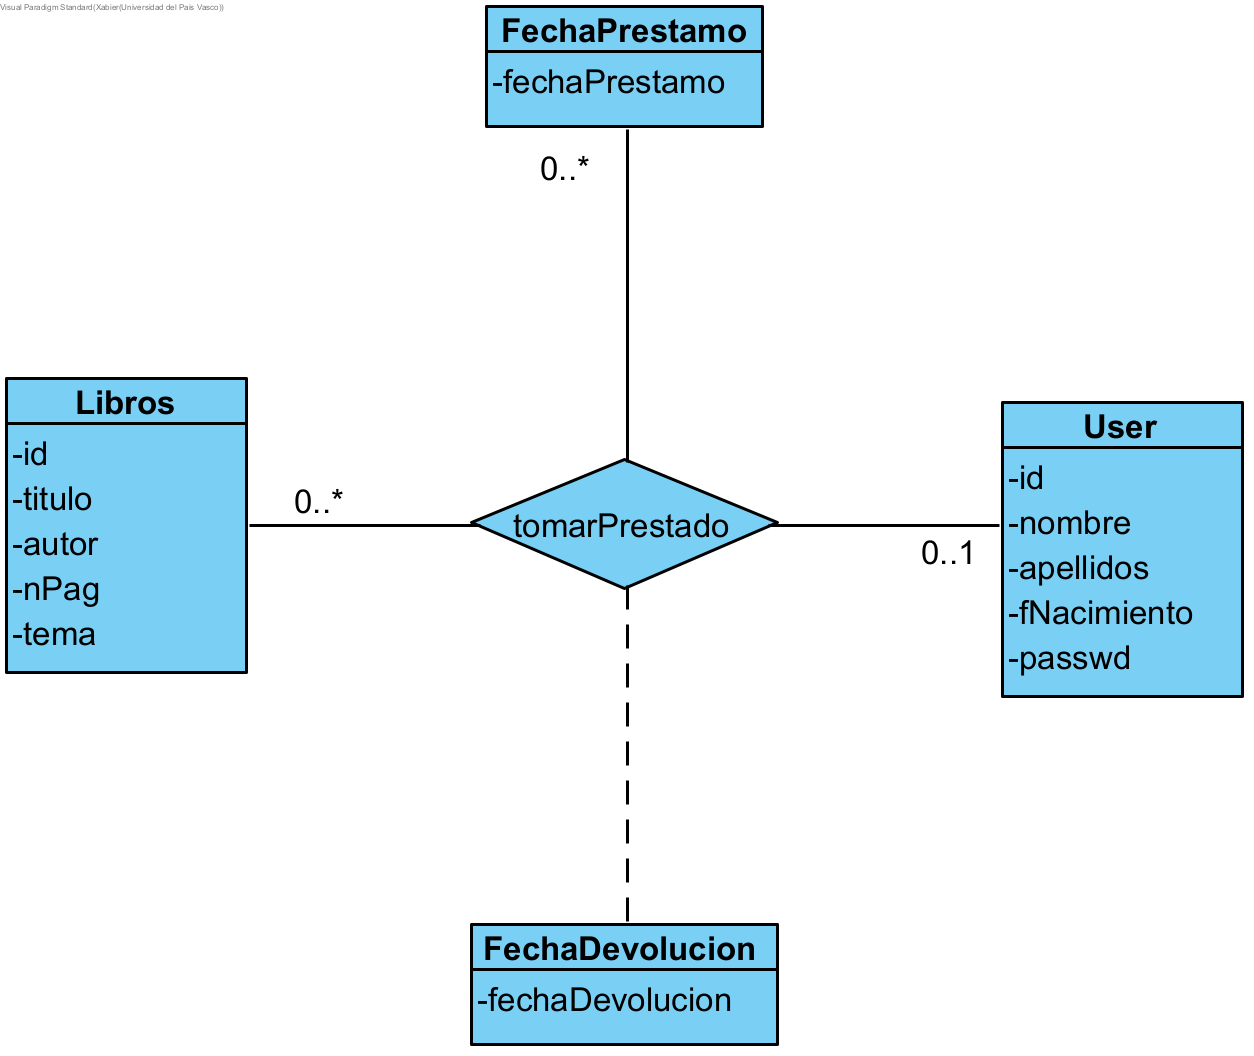
\includegraphics[width=1.0\textwidth]{img/dominio/tomarPrestado.png}
                        \caption{Diagrama de modelo de dominio de la relación tomarPrestado}
                    \end{figure}
                \clearpage
                \subsubsection{escribirReseña}
                    Esta relacion es la que permite guardar la reseña que un usuario pueda escribir en un libro. Al solo tener el atributo Reseña el usuario solo puede escribir una unica reseña sobre un libro.
                    \begin{figure}[H]
                        \centering
                        \includegraphics[width=1.0\textwidth]{img/dominio/escribirReseña.png}
                        \caption{Diagrama de modelo de dominio de la relación escribirReseña}
                    \end{figure}
                \clearpage
                \subsubsection{amistad}
                    La relacion amistad es la que permite que los usuarios puedan tener amigos en el sistema y guardar dichas amistades. 
                    \begin{figure}[H]
                        \centering
                        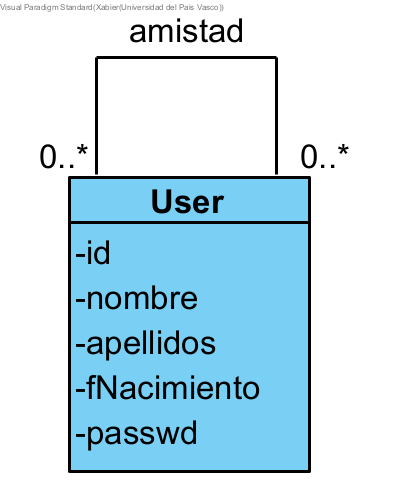
\includegraphics[width=0.5\textwidth]{img/dominio/amistad.png}
                        \caption{Diagrama de modelo de dominio de la relación amistad}
                    \end{figure}
                \clearpage
                \subsubsection{responderHilo}
                    Esta relacion permite que los usuarios puedan responder a los hilos del foro. La entidad fechaHoraRespuesta es la encargada de diferenciar las respuestas de un mismo usuario en un mismo hilo.
                    \begin{figure}[H]
                        \centering
                        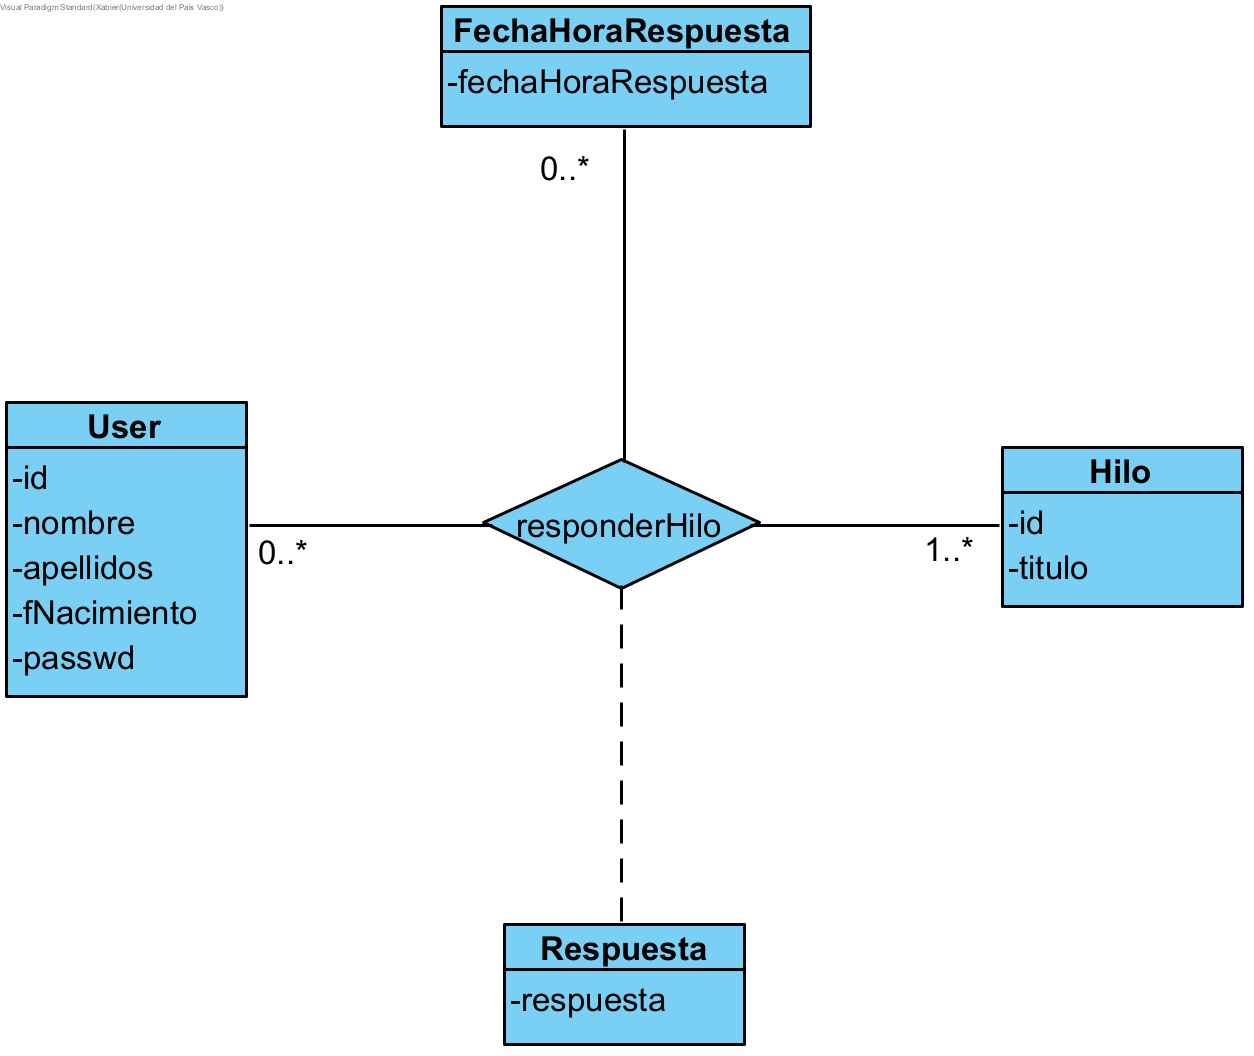
\includegraphics[width=1.0\textwidth]{img/dominio/responderHilo.png}
                        \caption{Diagrama de modelo de dominio de la relación responderHilo}
                    \end{figure}
                \clearpage
                \subsubsection{crearHilo}
                    Esta relacion almacena los datos de creacion de un hilo en el sistema. El sistema guardara el usuario que crea el hilo y en que fecha lo crea. Los hilos son unicos y para evitar repeticiones hacemos que sean unicos por lo que no guardamos la fecha como entidad si no como atributo de la relacion.
                    \begin{figure}[H]
                        \centering
                        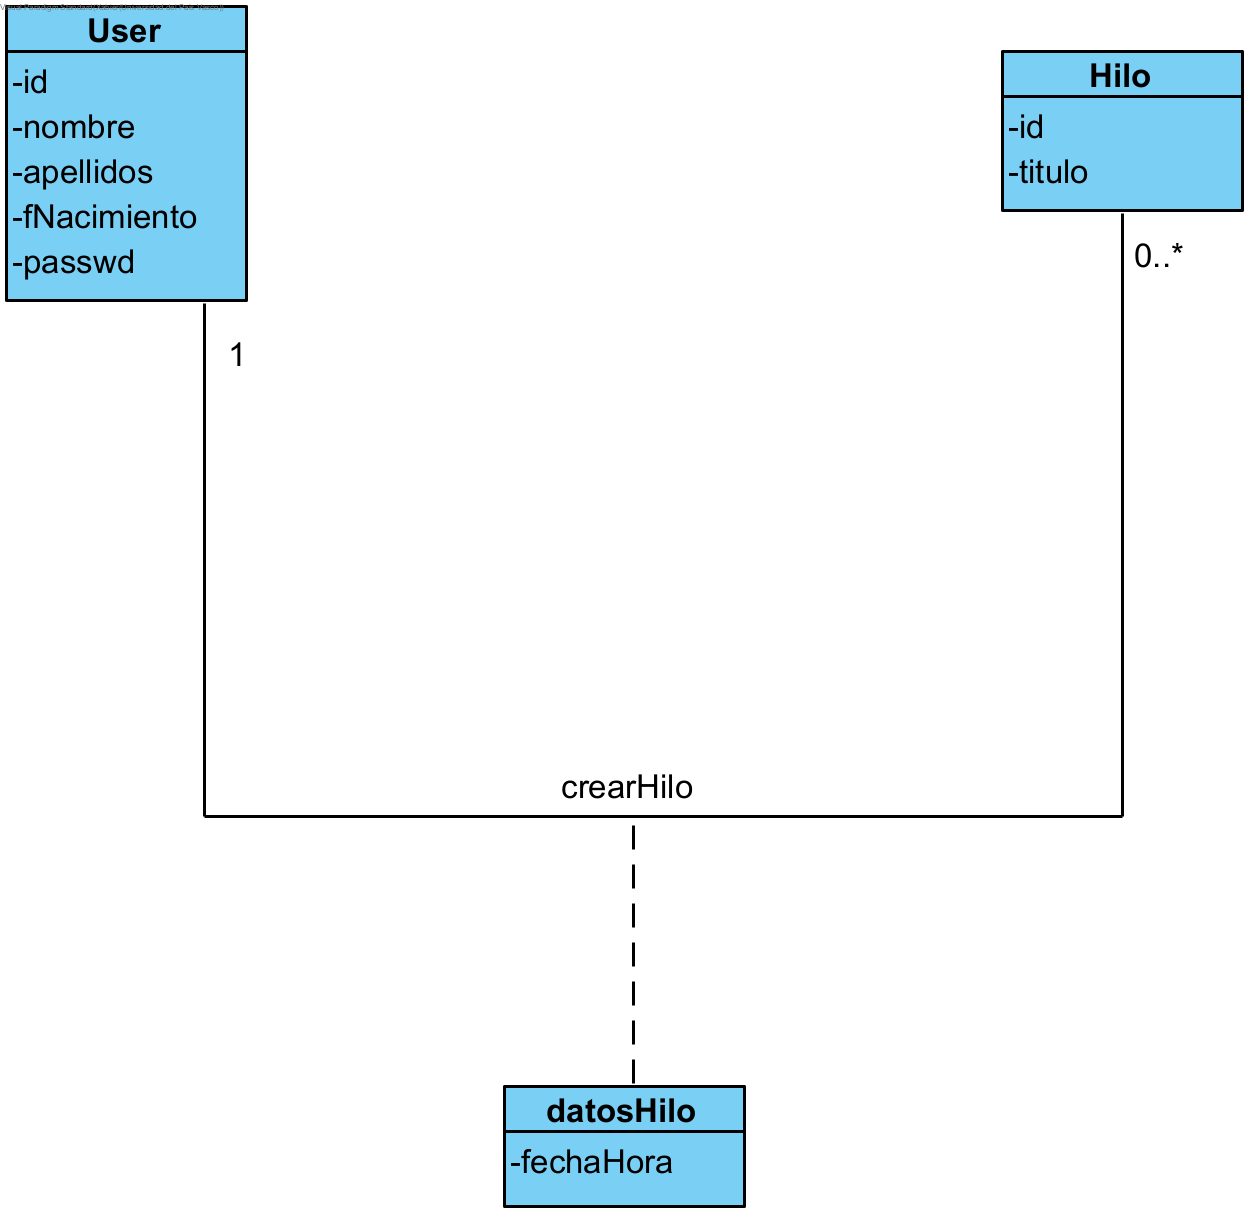
\includegraphics[width=0.7\textwidth]{img/dominio/crearHilo.png}
                        \caption{Diagrama de modelo de dominio de la relación crearHilo}
                    \end{figure}
                \clearpage
                \subsubsection{crean}
                    Esta relacion almacena los datos de creacion de los usuarios y de los libros por parte de un administrados.
                    \begin{figure}[H]
                        \centering
                        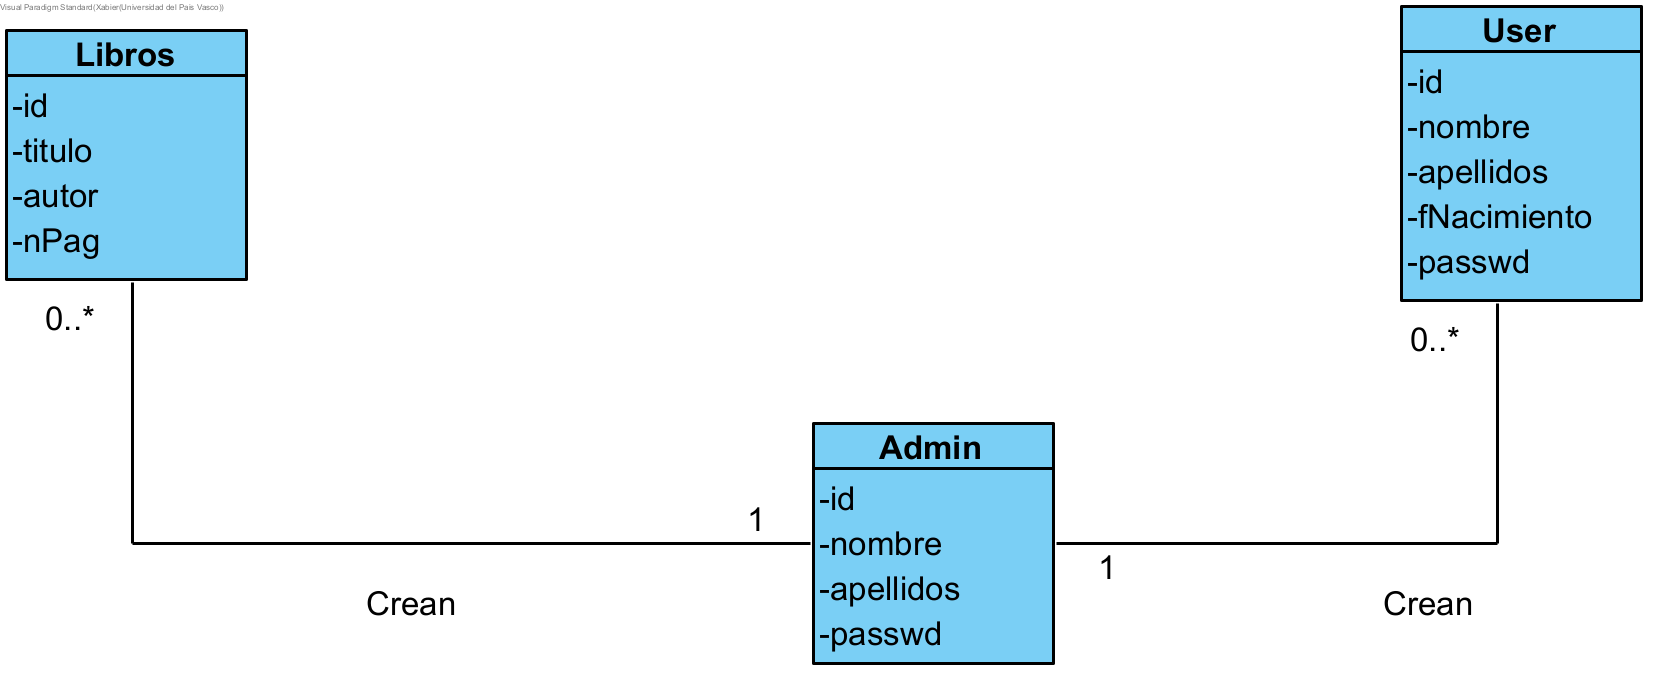
\includegraphics[width=0.7\textwidth]{img/dominio/crean.png}
                        \caption{Diagrama de modelo de dominio de la relación crean}
                    \end{figure}
                \clearpage
                \subsubsection{copiaDe}
                    Esta relacion almacena los datos de las copias de los libros que hay en el sistema. La entidad copiaLibros es la encargada de diferenciar las copias de un mismo libro.
                    \begin{figure}[H]
                        \centering
                        \includegraphics[width=0.7\textwidth]{img/dominio/copiaDe.png}
                        \caption{Diagrama de modelo de dominio de la relación copiaDe}
                    \end{figure}
    \chapter{Plan de Pruebas}
        \section{Gestión de reservas}
            \begin{center}
                \textbf{Responsable:} Kepa Reches Urrutia\\
                \begin{longtable}{|m{2cm}|m{4cm}|m{4cm}|}
                    \hline
                    Codigo & Descripción & Resultado esperado \\
                    \hline
                    \endhead \hline
                    F1P1 & El usuario selecciona un libro y pulsa reservar & Muestra la interfaz de reserva  \\
                    \hline
                    F1P1.2 & El usuario selecciona un libro y NO pulsa reservar  & Se mantiene en la interfaz del catálogo  \\
                    \hline
                    F1P2 & El usuario selecciona una fecha menor de 2 meses & La reserva es correcta  \\
                    \hline
                    F1P2.2 & El usuario selecciona una fecha mayor de 2 meses &  Se abre una interfaz de error en la reserva \\
                    \hline
                    F1P2.3 & El usuario no selecciona ninguna fecha & Se abre una interfaz de error en la reserva   \\
                    \hline          
                \end{longtable}
            \end{center}
            \clearpage
        \section{Reseñas}
            \begin{center}
                \textbf{Responsable:} Mohamed El Basri Dehbi\\
                \begin{longtable}{|m{2cm}|m{4cm}|m{4cm}|}
                    \hline
                    Codigo & Descripción & Resultado esperado \\
                    \hline
                    \endhead
                    \hline
                    F2P1 & Agregar reseña y puntuación a un libro & La reseña y puntuación se registran correctamente \\
                    \hline
                    F2P1.1 & Modificar reseña y puntuación de un libro & La reseña y puntuación se actualizan correctamente \\
                    \hline
                    F2P2 & Intentar agregar reseña y puntuación sin devolver el libro & Se muestra un mensaje de error \\
                    \hline
                    F2P3 & Ver reseña y puntuación de un libro & La reseña y puntuación del libro son visibles \\
                    \hline
                    F2P4 & Cambiar reseña y puntuación después de devolver el libro & La reseña y puntuación se pueden cambiar \\
                    \hline
                    F2P5 & Ver reseña y puntuación de otro usuario & La reseña y puntuación del usuario son visibles \\
                    \hline
                    F2P6 & Ver reseña y puntuación de un libro sin reseñas & Sistema muestra un mensaje indicando la ausencia de reseñas \\
                    \hline
                \end{longtable}
            \end{center}
            \clearpage
        \section{Red de amigos} 
            \begin{center}
                \textbf{Responsable:} Javier Criado Garcia\\
                \begin{longtable}{|m{2cm}|m{4cm}|m{4cm}|}
                    \hline
                    Codigo & Descripción & Resultado esperado \\
                    \hline
                    \endhead 
                    \hline
                    F3P1 & Ver perfil con sesión iniciada & Muestra el perfil  \\
                    \hline
                    F3P2 & El usuario pulsa el botón “Editar perfil”  & Se habilitan los campos para editar el perfil   \\
                    \hline
                    F3P3 & El usuario pulsa el botón “Consultar reservas” & Se abre una interfaz donde ver las reservas   \\
                    \hline
                    F3P4 & El usuario pulsa el botón “Consultar reseñas” &  Se abre una interfaz donde ver las reseñas \\
                    \hline
                    F3P5 & El usuario pulsa el botón “Agregar amigo” & Se abre una interfaz donde añadir un amigo  \\
                    \hline
                    F3P5.1 & El usuario pulsa "OK" & El amigo introducido es añadido  \\
                    \hline
                    F3P6 & El usuario pulsa el botón “Solicitudes de amistad” & Se abre una interfaz donde ver las solicitudes de amistad  \\
                    \hline
                    F3P7 & El usuario pulsa el botón “Borrar amigo” & Se abre una interfaz donde eliminar un amigo   \\
                    \hline  
                    F3P7.1 & El usuario pulsa "SI"  &  El amigo seleccionado es eliminado \\ 
                    \hline    
                    F3P7.2 & El usuario pulsa "NO"  &  El amigo seleccionado no es eliminado \\ 
                    \hline          
                \end{longtable}
            \end{center}
            \clearpage
        \section{Administrador}
            \begin{center}
                \textbf{Responsable:} Jon Valdes Granado\\
                \begin{longtable}{|m{2cm}|m{4cm}|m{4cm}|}
                    \hline
                    Codigo & Descripción & Resultado esperado \\
                    \hline
                    \endhead 
                    \hline
                    F4P1 & El usuario accede como administrador al sistema & Muestra la interfaz de menú del administrador  \\
                    \hline
                    F4P2 & El usuario pulsa el botón “Usuarios”  & Muestra la interfaz de gestión de usuario   \\
                    \hline
                    F4P3 & El usuario pulsa el botón “Crear” & Muestra la interfaz de creación de usuario   \\
                    \hline
                    F4P3.1 & El usuario introduce todos los campos correctamente y pulsa el botón "Crear" &  Se crea un nuevo usuario correctamente \\
                    \hline
                    F4P3.2 & El usuario introduce algún campo erróneo o no introduce alguno & Se mostrará un error por pantalla  \\
                    \hline
                    F4P4 & El usuario pulsa el botón “Editar” & Muestra la interfaz de edición de usuario \\
                    \hline
                    F4P4.1 & El usuario introduce todos los campos correctamente y pulsa el botón "Crear" &  Se edita el usuario correctamente  \\
                    \hline
                    F4P4.2 & El usuario introduce algún campo erróneo o no introduce alguno & Se mostrará un error por pantalla   \\
                    \hline  
                    F4P5 & El usuario pulsa el botón “Borrar” & Muestra la interfaz de eliminación de usuario \\ 
                    \hline    
                    F4P5.1 & El usuario introduce el correo electrónico del usuario correctamente y pulsa el botón "Borrar" &  Se borra el usuario correctamente \\ 
                    \hline
                    F4P5.2 & El usuario introduce un correo electrónico inexistente en el sistema & Se mostrará un error por pantalla \\ 
                    \hline 
                \end{longtable}
            \end{center}
            \clearpage
        \section{Foros}
            \begin{center}
                \textbf{Responsable:} Janire Veganzones García\\
                \begin{longtable}{|m{2cm}|m{4cm}|m{4cm}|}
                    \hline
                    Codigo & Descripción & Resultado esperado \\
                    \hline
                    \endhead
                    \hline
                    F5P1 & El usuario pulsa la opción ``Foro" de la cabecera & Se muestra la interfaz principal del foro con todo los hilos creados y con el botón para poder crear uno nuevo \\
                    \hline
                     F5P2 & El usuario pulsa el botón ``+Hilo" & Se muestra la interfaz de crear un hilo \\
                    \hline
                     F5P2.1 & El usuario pulsa el botón ``Cancelar" & No se crea ningún hilo y te redirecciona a la pantalla principal del foro \\
                    \hline
                     F5P2.2 & El usuario introduce todos los campos correctamente y pulsa el botón ``+Hilo" &  Se crea un Hilo correctamente y te redirecciona a la pantalla principal del foro donde lo podrás comprobar\\
                    \hline
                     F5P2.3 & El usuario introduce todos los campos excepto nombre & Se mostrará un mensaje de error por pantalla \\
                    \hline
                    F5P2.4 & El usuario introduce todos los campos excepto descripción & Se mostrará un mensaje de error por pantalla \\
                    \hline
                    F5P2.5 & El usuario introduce todos los campos excepto mensaje & Se mostrará un mensaje de error por pantalla \\
                    \hline
                    F5P3 & EL usuario pulsa sobre el hilo que quiere leer & Se mostrará la interfaz con los mensajes escritos por cada persona hasta ahora y con un botón para poder escribir un mensaje \\
                    \hline
                    F5P3.1 & El usuario pulsa el botón  ``+Mensaje" & Se mostrará una interfaz donde podrás escribir tú mensaje para posteriormente publicarlo en el hilo \\
                    \hline
                    F5P3.1.1 & El usuario escribe un mensaje y pulsa el botón ``Enviar" & Te redirecciona a la pantalla anterior donde se pueden ver los mensaje y comprobar que tu mensaje ha sido publicado correctamente \\
                    \hline
                    F5P3.1.2 & El usuario pulsa el botón "Enviar" sin escribir ningún mensaje & Se mostrará un mensaje de error por pantalla  \\
                    \hline
                \end{longtable}
            \end{center}
            \clearpage
        \section{Recomendaciones del sistema}
            \begin{center}
                \textbf{Responsable:} Ainhize Martinez Duran\\
                \begin{longtable}{|m{2cm}|m{4cm}|m{4cm}|}
                    \hline
                    Codigo & Descripción & Resultado esperado \\
                    \hline
                    \endhead
                    \hline
                    F6.P1 & Entrar en el catálogo sin haber iniciado sesión & Muestra el catálogo pero no mostrará ninguna recomendación \\
                    \hline
                    F6.P2 & Entrar en el catálogo habiendo iniciado sesión pero sin haber hecho ninguna reserva & Muestra el catálogo pero no mostrará ninguna recomendación \\
                    \hline
                    F6.P3 & Entrar en el catálogo habiendo iniciado sesión y reservado un único libro & Muestra el catálogo y las recomendaciones asociadas al único libro que ha reservado \\
                    \hline
                    F6.P3.1 & Entrar en el catálogo habiendo iniciado sesión y reservado el único libro que existe de un tema & Muestra el catálogo pero no mostrará ninguna recomendación \\
                    \hline
                    F6.P4 & Entrar en el catálogo habiendo iniciado sesión y reservado varios libros & Muestra el catálogo y las recomendaciones asociadas a los libros que ha reservado \\
                    \hline
                \end{longtable}
            \end{center}
            \clearpage
        \section{Recomendaciones de amigos}
            \begin{center}
                \textbf{Responsable:} Xabier Gabiña Barañano\\
                \begin{longtable}{|m{2cm}|m{4cm}|m{4cm}|}
                    \hline
                    Codigo & Descripción & Resultado esperado \\
                    \hline
                    \endhead
                    \hline
                    F7P1 & Ver perfil sin iniciar sesion & Muestra el perfil sin recomendaciones \\
                    \hline
                    F7P1.1 & Ver otro perfil al de la sesion & Muestra el otro perfil sin recomendaciones \\
                    \hline
                    F7P2 & Ver perfil con sesion pero sin amigos ni libros alquilados previamente/actualmente & Muestra el perfil sin recomendaciones \\
                    \hline
                    F7P3 & Ver perfil con sesion y amigos pero sin libros alquilados previamente/actualmente & Muestra el perfil sin recomendaciones con recomendaciones basadas en los amigos \\
                    \hline
                    F7P3.1 & Ver perfil con sesion y amigos pero sin libros alquilados previamente/acutlamente y tus amigos no tienen otros amigos & Muestra el perfil sin recomendaciones \\
                    \hline
                    F7P4 & Ver perfil con sesion y libros alquilados previamente/actualmente pero sin amigos & Muestra las recomendaciones en base a los libros aliquilados previamente/actualmente \\
                    \hline
                    F7P4.1 & Ver perfil con sesion y libros alquilados perviamente/actualmente pero sin amigos y el libro es el unico de su tema & Muestra el perfil sin recomendaciones \\
                    \hline
                    F7P5 & Ver perfil con sesion, amigos y libros alquilados previamente/actualmente & Muestra las recomendaciones en base a los libros alquilados previamente/actualmente y los amigos \\
                    \hline
                \end{longtable}
            \end{center}
            \clearpage
    \chapter{Diagrama relacional}
        \begin{figure}[H]
            \centering
            \includegraphics[width=1.0\textwidth]{img/relacional/relacional.png}
            \caption{Diagrama relacional}
        \end{figure}
    \chapter{Diagrama de clases}
        \begin{figure}[H]
            \centering
            \includegraphics[width=1.0\textwidth]{img/clases/clases.png}
            \caption{Diagrama de clases}
        \end{figure}
    \chapter{Diagramas de comunicación}
        \section{Gestión de reservas}
            \textbf{Mohamed El Basri}
            \begin{figure}[H]
                \centering
                %\includegraphics[width=1.0\textwidth]{img/comunicacion/gestionDeReservas.png}
                \caption{Diagrama de comunicación de la gestión de reservas}
            \end{figure}
            \clearpage
        \section{Reseñas}
            \textbf{Javier Criado Garcia}
            \begin{figure}[H]
                \centering
                %\includegraphics[width=1.0\textwidth]{img/comunicacion/resenas.png}
                \caption{Diagrama de comunicación de las reseñas}
            \end{figure}
            \clearpage
        \section{Red de amigos}
            \textbf{Jon Valdes Granado}
            \begin{figure}[H]
                \centering
                %\includegraphics[width=1.0\textwidth]{img/comunicacion/redDeAmigos.png}
                \caption{Diagrama de comunicación de la red de amigos}
            \end{figure}
            \clearpage
        \section{Administrador}
            \textbf{Janire Veganzones García}
            \begin{figure}[H]
                \centering
                \includegraphics[width=1.0\textwidth]{img/comunicacion/Diagrama1.png}
                \caption{Diagrama de comunicación general del administrador}
            \clearpage
            \begin{enumerate}
                \item El usuario inicia sesión como Admin.
                \item new ilustration\_3.2.4.1.2().
                \item Pulsa ``Usuarios''.
                \item new ilustration\_3.2.4.1.3().
                \item Pulsa ``Libros''.
                \item new ilustration\_3.2.4.2.3().
            \end{enumerate}
            \end{figure}
            \clearpage
                        \begin{figure}[H]
                \centering
                \includegraphics[width=1.15\textwidth]{img/comunicacion/diagrama2.png}
                \caption{Diagrama de comunicación Crear un Usuario}
            \clearpage
            \begin{enumerate}
                \item El usuario pulsa ``Crear''.
                \item new ilustration\_3.2.4.1.4().
                \item Introducir nombre, apellidos, fecha nacimiento, email, contraseña y contraseña2 y pulsar ``Crear''.
                \item comprobarDatosRegistro(nombre, apellidos, fecha\_nacimiento, passwd, passwd2, email) : boolean 
                \newline
                [Si comprobarDatosRegistro == TRUE]
                \item  crear(nombre, apellidos, fecha\_nacimiento, email, passwd): void
                \begin{enumerate}
                    \item[5.1]  crear(nombre, apellidos, fecha\_nacimiento, email, passwd): void
                        \begin{enumerate}
                            \item[5.1.1] execSQL (INSERT INTO User VALUES (\%nombre\%, \%apellidos\%, \%fecha\_nacimiento\%, \%email\%, \%passwd\% ) ): ResultadoSQL
                        \end{enumerate}
                    \end{enumerate}
                    [Si No]
                \item new ilustration\_3.2.4.1.5().
            \end{enumerate}
            \end{figure}
            
            \begin{figure}[H]
                \centering
                \includegraphics[width=1.1\textwidth]{img/comunicacion/diagrama3.png}
                \caption{Diagrama de comunicación Borrar un Usuario}
            \clearpage
            \begin{enumerate}
                \item El usuario pulsa ``Borrar''.
                \item new ilustration\_3.2.4.1.6().
                \item Escribir el email del usuario que desees eliminar y pulsar ``Borrar''.
                \item usuarioBuscado = encontrarUser(email): int
                \begin{enumerate}
                    \item[4.1] encontrarUser(email)
                        \begin{enumerate}
                            \item[4.1.1] execSQL( SELECT id\_user FROM User WHERE email = \%email\%): ResultadoSQL
                                \begin{enumerate}
                                    \item[4.1.1.1] new ResultadoSQL()
                                \end{enumerate}
                            \item[4.1.2] next()
                            \item[4.1.3] getInt(id\_user): int
                        \end{enumerate}
                \end{enumerate}
                [SI usuarioBuscado != NULL]
                \item eliminarUsuario(id\_user)
                 \begin{enumerate}
                    \item[5.1] eliminarUsuario(id\_user)
                        \begin{enumerate}
                            \item[5.1.1] execSQL( DELETE * FROM Reseña WHERE id\_user= usuarioBuscado ) 
                            \item[5.1.2] execSQL( DELETE * FROM Responder\_hilo WHERE id\_user= usuarioBuscado ) 
                            \item[5.1.3] execSQL( DELETE * FROM Tomar\_prestamo WHERE id\_user = usuarioBuscado ) 
                            \item[5.1.4] execSQL( DELETE * FROM User WHERE id\_user= UsuarioAElimiar) 
                        \end{enumerate}
                \end{enumerate}
                    [Si No]
                \item new ilustration\_3.2.4.1.7().
            \end{enumerate}
            \end{figure}
            \clearpage

            \begin{figure}[H]
                \centering
                \includegraphics[width=1.1\textwidth]{img/comunicacion/diagrama6.png}
                \caption{Diagrama de comunicación Modificar un Usuario}
            \clearpage
            \begin{enumerate}
                \item El usuario pulsa ``Modificar''.
                \item new ilustration\_3.2.4.1.8().
                \item Introducir Nombre, Apellidos, Fecha nacimiento, Email, Nuevo nombre, Nuevos Apellidos, Nueva fecha nacimiento, Nueva contraseña, Repetir nueva contraseña y pulsar ``Modificar''.
                \item encontrarUser(email) [Función desarrollada en el diagrama anterior]
                \newline
                [SI usuarioBuscado != NULL]
                \newline
                [SI \%Nueva contraseña\% == \%Repetir nueva contraseña\%]
                \item modificarUsuario(id\_user)
                \begin{enumerate}
                    \item[5.1] modificarUsuario(id\_user)
                        \begin{enumerate}
                            \item[5.1.1] execSQL(UPDATE User SET nombre = \%Nuevo nombre\%,\ apellidos = \%Nuevos apellidos\%, fecha\_nacimiento = \%Nueva fecha nacimiento\%, passwd = \%Nueva contraseña\% WHERE id\_user = id\_user)
                        \end{enumerate}
                    [Si No]
                \end{enumerate}
                \item new ilustration\_3.2.4.1.9().
                \newline
                [Si No]
                \item new ilustration\_3.2.4.1.9().
            \end{enumerate}
            \end{figure}
            \clearpage

                    \begin{figure}[H]
                \centering
                \includegraphics[width=1.1\textwidth]{img/comunicacion/Diagrama4.png}
                \caption{Diagrama de comunicación Insertar un Libro}
            \clearpage
            \begin{enumerate}
                \item El usuario pulsa ``Añadir''.
                \item new ilustration\_3.2.4.2.4().
                \item Rellenar los campos Título y autor y pulsar ``Insertar''.
                \item comprobarDatosLibro(título, autor): boolean 
                \newline
                [Si comprobarDatosLibro == TRUE]
                \item  añadirLibro(titulo,autor): void
                \begin{enumerate}
                    \item[5.1]  añadirLibro(titulo,autor): void
                        \begin{enumerate}
                            \item[5.1.1] exectSQL (INSERT INTO Libros (\%titulo\%, \%autor\%): ResultadoSQL
                        \end{enumerate}
                    \end{enumerate}
                    [Si No]
                \item new ilustration\_3.2.4.2.5().
            \end{enumerate}
            \end{figure}

            \begin{figure}[H]
                \centering
                \includegraphics[width=1.1\textwidth]{img/comunicacion/diagrama5.png}
                \caption{Diagrama de comunicación Borrar un Libro}
            \clearpage
            \begin{enumerate}
                \item El usuario pulsa ``Eliminar''.
                \item new ilustration\_3.2.4.2.6().
                \item Escribir el titulo y autor del libro que desees eliminar  y pulsar ``Eliminar''.
                \item libroBuscado= encontrarLibro(titulo): int
                \begin{enumerate}
                    \item[4.1] encontrarLibro(titulo)
                        \begin{enumerate}
                            \item[4.1.1] execSQL( SELECT id\_libro FROM Libro WHERE titulo = \%titulo\%): ResultadoSQL
                                \begin{enumerate}
                                    \item[4.1.1.1] new ResultadoSQL()
                                \end{enumerate}
                            \item[4.1.2] next()
                            \item[4.1.3] getInt(id\_libro): int
                        \end{enumerate}
                \end{enumerate}
                [SI libroBuscado != NULL]
                \item eliminarLibro(id\_libro)
                 \begin{enumerate}
                    \item[5.1] eliminarLibro(id\_libro)
                        \begin{enumerate}
                            \item[5.1.1] execSQL( DELETE * FROM Reseña WHERE id\_libro= libroBuscado) 
                            \item[5.1.2] execSQL( DELETE * FROM CopiaLibro WHERE id\_libro= libroBuscado) 
                            \item[5.1.3] execSQL( DELETE * FROM Libro WHERE id\_libro= libroBuscado) 
                        \end{enumerate}
                \end{enumerate}
                    [Si No]
                \item new ilustration\_3.2.4.2.7().
            \end{enumerate}
            \end{figure}
            \clearpage

        \begin{figure}[H]
                \centering
                \includegraphics[width=1.1\textwidth]{img/comunicacion/diagrama7.png}
                \caption{Diagrama de comunicación Modificar un Libro}
            \clearpage
            \begin{enumerate}
                \item El usuario pulsa ``Modificar''.
                \item new ilustration\_3.2.4.2.8().
                \item Introducir titulo anterior, autor anterior, titulo nuevo y autor nuevo y pulsar ``Modificar''.
                \item encontrarLibro(titulo) [Función desarrollada en el diagrama anterior]
                \newline
                [SI libroBuscado != NULL]
                \item modificarLibro(id\_libro)
                \begin{enumerate}
                    \item[5.1] modificarLibro(id\_libro)
                        \begin{enumerate}
                            \item[5.1.1] execSQL(UPDATE Libro SET titulo= \%titulo nuevo\%, autor= \%autor nuevo\%)
                        \end{enumerate}
                    [Si No]
                \end{enumerate}
                \item new ilustration\_3.2.4.2.9().
                \newline
                [Si No]
                \item new ilustration\_3.2.4.2.9().
            \end{enumerate}
            \end{figure}
            \clearpage
        \section{Foros}
            \textbf{Ainhize Martinez Duran}
            \begin{figure}[H]
                \centering
                %\includegraphics[width=1.0\textwidth]{img/comunicacion/foros.png}
                \caption{Diagrama de comunicación de los foros}
            \end{figure}
            \begin{verbatim}
                JSON_Hilo{
                    [
                        {
                            "id_hilo":int,
                            "titulo":String
                        }
                    ]
                }
            \end{verbatim}
            \begin{verbatim}
                JSON_Respuesta{
                    [
                        {
                            "mensaje":Strin,
                            "user":String
                        }
                    ]
                }
            \end{verbatim}
            \begin{enumerate}
                \item El usuario selecciona Foro en el menú principal.
                \item new Foro()
                \item getHilos():JSON\_Hilo
                \begin{enumerate}
                    \item [3.1] crearNuevoHilo(user\_id):JSON\_Hilo
                    \item [3.2] entrarHilo(id\_hilo):JSON\_Respuesta
                    \begin{enumerate}
                        \item [3.2.1] mo()
                    \end{enumerate}
                    \begin{enumerate}
                        \item [3.2.1.1] responderHilo()
                    \end{enumerate}
                \end{enumerate}
            \end{enumerate}
            \clearpage
        \section{Recomendaciones del sistema}
            \textbf{Xabier Gabiña Barañano}
            \begin{figure}[H]
                \centering
                \includegraphics[width=1.0\textwidth]{img/comunicacion/recomendacionesDelSistema.png}
                \caption{Diagrama de comunicación de las recomendaciones del sistema}
            \end{figure}
            \begin{verbatim}
                JSON_Libros{
                    [
                        {
                            "id_libro":int,
                            "nombre":String
                        }
                    ]
                }
            \end{verbatim}
            \clearpage
            \begin{enumerate}
                \item El usuario selecciona el catálogo en el menú principal.
                \item new UI\_CATALOGO(user\_id).
                \item getRecomendacionesUser(user\_id):JSON\_Libros
                \begin{enumerate}
                    \item[3.1] listaLibros=getUserData(user\_id):JSON\_Libros
                    \begin{enumerate}
                        \item[3.1.1] execSQL(''
                            SELECT Libro.* 
                            FROM User 
                            INNER JOIN Tomar\_prestamo ON User.id\_user = Tomar\_prestamo.id\_user
                            INNER JOIN CopiaLibro ON Tomar\_prestamo.id\_copia = CopiaLibro.id\_copia
                            INNER JOIN Libro ON CopiaLibro.id\_libro = Libro.id\_libro
                            WHERE User.id\_user = \%user\_id\%;
                            ''): ResultadoSQL
                        \begin{enumerate}
                            \item[3.1.1.1] new ResultadoSQL()
                        \end{enumerate}
                        \item[3.1.2] next()
                        \item[3.1.3] getInt('id\_libro'):int
                        \item[3.1.4] getString('nombre'):String
                    \end{enumerate}
                    \item[3.2] listaLibros=getFriendsData(user\_id):JSON\_Libros
                    \begin{enumerate}
                        \item[3.2.1] execSQL(''
                            SELECT Libro.* 
                            FROM User 
                            INNER JOIN Amistad ON User.id\_user = Amistad.id\_user1
                            INNER JOIN User Amigo ON Amistad.id\_user2 = Amigo.id\_user
                            INNER JOIN Tomar\_prestamo ON Amigo.id\_user = Tomar\_prestamo.id\_user
                            INNER JOIN CopiaLibro ON Tomar\_prestamo.id\_copia = CopiaLibro.id\_copia
                            INNER JOIN Libro ON CopiaLibro.id\_libro = Libro.id\_libro
                            WHERE User.id\_user = \%user\_id\%;
                            ''): ResultadoSQL
                        \begin{enumerate}
                            \item[3.2.1.1] new ResultadoSQL()
                        \end{enumerate}
                        \item[3.2.2] next()
                        \item[3.2.3] getInt('id\_libro'):int
                        \item[3.2.4] getString('nombre'):String
                    \end{enumerate}
                    \item[3.3] getRecomendaciones(listaLibros):JSON\_Libros
                    \begin{enumerate}
                        \item[3.3.1] execSQL(''
                            SELECT Libro.*
                            FROM Libro
                            INNER JOIN Pertenece ON Libro.id\_libro = Pertenece.id\_libro
                            INNER JOIN Tema ON Pertenece.id\_tema = Tema.id\_tema
                            WHERE Tema.id\_tema IN (
                                SELECT Pertenece.id\_tema
                                FROM Pertenece
                                WHERE Pertenece.id\_libro = \%libro\_id\%
                                );
                            ''): ResultadoSQL
                        \begin{enumerate}
                            \item[3.3.1.1] new ResultadoSQL()
                        \end{enumerate}
                        \item[3.3.2] next()
                        \item[3.3.3] getInt('id\_libro'):int
                        \item[3.3.4] getString('nombre'):String
                    \end{enumerate}
                \end{enumerate}
            \end{enumerate}
            \clearpage
        \section{Recomendaciones de amigos}
            \textbf{Kepa Reche Urrutia}
            \begin{figure}[H]
                \centering
                %\includegraphics[width=1.0\textwidth]{img/comunicacion/recomendacionesDeAmigos.png}
                \caption{Diagrama de comunicación de las recomendaciones de amigos}
            \end{figure}
            \clearpage
\end{document}
